\documentclass[ twoside,openright,titlepage,numbers=noenddot,headinclude,%1headlines,% letterpaper a4paper
                footinclude=true,cleardoublepage=empty,abstractoff, % <--- obsolete, remove (todo)
                BCOR=5mm,paper=a4,fontsize=11pt,%11pt,a4paper,%
                ngerman,american,%
                ]{scrreprt}


%load fonts und useful packages. etc.
% ****************************************************************************************************
% classicthesis-config.tex 
% formerly known as loadpackages.sty, classicthesis-ldpkg.sty, and classicthesis-preamble.sty 
% Use it at the beginning of your ClassicThesis.tex, or as a LaTeX Preamble 
% in your ClassicThesis.{tex,lyx} with \input{classicthesis-config}
% ****************************************************************************************************  
% If you like the classicthesis, then I would appreciate a postcard. 
% My address can be found in the file ClassicThesis.pdf. A collection 
% of the postcards I received so far is available online at 
% http://postcards.miede.de
% ****************************************************************************************************

% ****************************************************************************************************
% 1. Configure classicthesis for your needs here, e.g., remove "drafting" below 
% in order to deactivate the time-stamp on the pages
% ****************************************************************************************************
\PassOptionsToPackage{eulerchapternumbers,listings,drafting,%
				 pdfspacing,%floatperchapter,%linedheaders,%
				 subfig,beramono,eulermath}{classicthesis}										
% ********************************************************************
% Available options for classicthesis.sty 
% (see ClassicThesis.pdf for more information):
% drafting
% parts nochapters linedheaders
% eulerchapternumbers beramono eulermath pdfspacing minionprospacing
% tocaligned dottedtoc manychapters
% listings floatperchapter subfig
% ********************************************************************

% ********************************************************************
% Triggers for this config
% ******************************************************************** 
\usepackage{ifthen}
\newboolean{enable-backrefs} % enable backrefs in the bibliography
\setboolean{enable-backrefs}{false} % true false
% ****************************************************************************************************


% ****************************************************************************************************
% 2. Personal data and user ad-hoc commands
% ****************************************************************************************************
\newcommand{\myTitle}{Rotary Flexible Joint\xspace}
\newcommand{\mySubtitle}{ Project Report\xspace}
\newcommand{\myDegree}{\xspace}
\newcommand{\myName}{Matthias Baeten and Moritz Wolter\xspace}
\newcommand{\myProf}{Prof. Bart de Moor \xspace}
\newcommand{\myOtherProf}{Mauricio Agudelo  \xspace}
\newcommand{\mySupervisor}{\xspace}
\newcommand{\myFaculty}{\xspace}
\newcommand{\myDepartment}{\xspace}
\newcommand{\myUni}{KU Leuven\xspace}
\newcommand{\myLocation}{Leuven\xspace}
\newcommand{\myTime}{	\selectlanguage{american}
			\today \xspace}
\newcommand{\myVersion}{Version 1\xspace}

% ********************************************************************
% Setup, finetuning, and useful commands
% ********************************************************************
\newcounter{dummy} % necessary for correct hyperlinks (to index, bib, etc.)
\newlength{\abcd} % for ab..z string length calculation
\providecommand{\mLyX}{L\kern-.1667em\lower.25em\hbox{Y}\kern-.125emX\@}
\newcommand{\ie}{i.\,e.}
\newcommand{\Ie}{I.\,e.}
\newcommand{\eg}{e.\,g.}
\newcommand{\Eg}{E.\,g.} 
% ****************************************************************************************************


% ****************************************************************************************************
% 3. Loading some handy packages
% ****************************************************************************************************
% ******************************************************************** 
% Packages with options that might require adjustments
% ******************************************************************** 
\PassOptionsToPackage{utf8}{inputenc}	% latin9 (ISO-8859-9) = latin1+"Euro sign"
 \usepackage{inputenc}				

\PassOptionsToPackage{english}{babel}   % change this to your language(s)
% Spanish languages need extra options in order to work with this template
%\PassOptionsToPackage{spanish,es-lcroman}{babel}
 \usepackage{babel}					

 %\PassOptionsToPackage{square,numbers}{natbib}
 %\usepackage{natbib}
 \usepackage[fixlanguage]{babelbib}
 \selectbiblanguage{german}
 \bibliographystyle{babplain}

\PassOptionsToPackage{fleqn}{amsmath}		% math environments and more by the AMS 
 \usepackage{amsmath}

%When using tikZ one must also use the color package.
\PassOptionsToPackage{usenames,dvipsnames}{color}
 \usepackage{color}

%This package lets you compile tikz graphics.
 \usepackage{tikz}
 \usepackage{pgfplots}
 \usetikzlibrary{decorations.markings}
 \usepackage{standalone}

% ******************************************************************** 
% General useful packages
% ******************************************************************** 
\PassOptionsToPackage{T1}{fontenc} % T2A for cyrillics
	\usepackage{fontenc}     
\usepackage{textcomp} % fix warning with missing font shapes
\usepackage{scrhack} % fix warnings when using KOMA with listings package          
\usepackage{xspace} % to get the spacing after macros right  
\usepackage{mparhack} % get marginpar right
\usepackage{fixltx2e} % fixes some LaTeX stuff 
\PassOptionsToPackage{printonlyused,smaller}{acronym}
	\usepackage{acronym} % nice macros for handling all acronyms in the thesis
%\renewcommand*{\acsfont}[1]{\textssc{#1}} % for MinionPro
\renewcommand{\bflabel}[1]{{#1}\hfill} % fix the list of acronyms
% ****************************************************************************************************


% ****************************************************************************************************
% 4. Setup floats: tables, (sub)figures, and captions
% ****************************************************************************************************
\usepackage{tabularx} % better tables
	\setlength{\extrarowheight}{3pt} % increase table row height
\newcommand{\tableheadline}[1]{\multicolumn{1}{c}{\spacedlowsmallcaps{#1}}}
\newcommand{\myfloatalign}{\centering} % to be used with each float for alignment
\usepackage{caption}
\captionsetup{format=hang,font=small}
\usepackage{subfig}  
% ****************************************************************************************************


% ****************************************************************************************************
% 5. Setup code listings
% ****************************************************************************************************
\usepackage{listings} 
%\lstset{emph={trueIndex,root},emphstyle=\color{BlueViolet}}%\underbar} % for special keywords
\lstset{language=[LaTeX]Tex,%C++,
    keywordstyle=\color{RoyalBlue},%\bfseries,
    basicstyle=\small\ttfamily,
    %identifierstyle=\color{NavyBlue},
    commentstyle=\color{Green}\ttfamily,
    stringstyle=\rmfamily,
    numbers=none,%left,%
    numberstyle=\scriptsize,%\tiny
    stepnumber=5,
    numbersep=8pt,
    showstringspaces=false,
    breaklines=true,
    frameround=ftff,
    frame=single,
    belowcaptionskip=.75\baselineskip
    %frame=L
} 
% ****************************************************************************************************    		   


% ****************************************************************************************************
% 6. PDFLaTeX, hyperreferences and citation backreferences
% ****************************************************************************************************
% ********************************************************************
% Using PDFLaTeX
% ********************************************************************
\PassOptionsToPackage{pdftex,hyperfootnotes=false,pdfpagelabels}{hyperref}
	\usepackage{hyperref}  % backref linktocpage pagebackref
\pdfcompresslevel=9
\pdfadjustspacing=1 
\PassOptionsToPackage{pdftex}{graphicx}
	\usepackage{graphicx} 

% ********************************************************************
% Setup the style of the backrefs from the bibliography
% (translate the options to any language you use)
% ********************************************************************
\newcommand{\backrefnotcitedstring}{\relax}%(Not cited.)
\newcommand{\backrefcitedsinglestring}[1]{(Cited on page~#1.)}
\newcommand{\backrefcitedmultistring}[1]{(Cited on pages~#1.)}
\ifthenelse{\boolean{enable-backrefs}}%
{%
		\PassOptionsToPackage{hyperpageref}{backref}
		\usepackage{backref} % to be loaded after hyperref package 
		   \renewcommand{\backreftwosep}{ and~} % separate 2 pages
		   \renewcommand{\backreflastsep}{, and~} % separate last of longer list
		   \renewcommand*{\backref}[1]{}  % disable standard
		   \renewcommand*{\backrefalt}[4]{% detailed backref
		      \ifcase #1 %
		         \backrefnotcitedstring%
		      \or%
		         \backrefcitedsinglestring{#2}%
		      \else%
		         \backrefcitedmultistring{#2}%
		      \fi}%
}{\relax}    

% ********************************************************************
% Hyperreferences
% ********************************************************************
\hypersetup{%
    %draft,	% = no hyperlinking at all (useful in b/w printouts)
    colorlinks=true, linktocpage=true, pdfstartpage=3, pdfstartview=FitV,%
    % uncomment the following line if you want to have black links (e.g., for printing)
    %colorlinks=false, linktocpage=false, pdfborder={0 0 0}, pdfstartpage=3, pdfstartview=FitV,% 
    breaklinks=true, pdfpagemode=UseNone, pageanchor=true, pdfpagemode=UseOutlines,%
    plainpages=false, bookmarksnumbered, bookmarksopen=true, bookmarksopenlevel=1,%
    hypertexnames=true, pdfhighlight=/O,%nesting=true,%frenchlinks,%
    urlcolor=webbrown, linkcolor=RoyalBlue, citecolor=webgreen, %pagecolor=RoyalBlue,%
    %urlcolor=Black, linkcolor=Black, citecolor=Black, %pagecolor=Black,%
    pdftitle={\myTitle},%
    pdfauthor={\textcopyright\ \myName, \myUni, \myFaculty},%
    pdfsubject={},%
    pdfkeywords={},%
    pdfcreator={pdfLaTeX},%
    pdfproducer={LaTeX with hyperref and classicthesis}%
}   

% ********************************************************************
% Setup autoreferences
% ********************************************************************
% There are some issues regarding autorefnames
% http://www.ureader.de/msg/136221647.aspx
% http://www.tex.ac.uk/cgi-bin/texfaq2html?label=latexwords
% you have to redefine the makros for the 
% language you use, e.g., american, ngerman
% (as chosen when loading babel/AtBeginDocument)
% ********************************************************************
\makeatletter
\@ifpackageloaded{babel}%
    {%
       \addto\extrasamerican{%
					\renewcommand*{\figureautorefname}{Figure}%
					\renewcommand*{\tableautorefname}{Table}%
					\renewcommand*{\partautorefname}{Part}%
					\renewcommand*{\chapterautorefname}{Chapter}%
					\renewcommand*{\sectionautorefname}{Section}%
					\renewcommand*{\subsectionautorefname}{Section}%
					\renewcommand*{\subsubsectionautorefname}{Section}% 	
				}%
       \addto\extrasngerman{% 
					\renewcommand*{\paragraphautorefname}{Absatz}%
					\renewcommand*{\subparagraphautorefname}{Unterabsatz}%
					\renewcommand*{\footnoteautorefname}{Fu\"snote}%
					\renewcommand*{\FancyVerbLineautorefname}{Zeile}%
					\renewcommand*{\theoremautorefname}{Theorem}%
					\renewcommand*{\appendixautorefname}{Anhang}%
					\renewcommand*{\equationautorefname}{Gleichung}%        
					\renewcommand*{\itemautorefname}{Punkt}%
				}%	
			% Fix to getting autorefs for subfigures right (thanks to Belinda Vogt for changing the definition)
			\providecommand{\subfigureautorefname}{\figureautorefname}%  			
    }{\relax}
\makeatother


% ****************************************************************************************************
% 7. Last calls before the bar closes
% ****************************************************************************************************
% ********************************************************************
% Development Stuff
% ********************************************************************
\listfiles
%\PassOptionsToPackage{l2tabu,orthodox,abort}{nag}
%	\usepackage{nag}
%\PassOptionsToPackage{warning, all}{onlyamsmath}
%	\usepackage{onlyamsmath}

% ********************************************************************
% Last, but not least... 
% ********************************************************************
\usepackage{classicthesis} 
% Die guten TU-Farben...
\renewcommand\cftchapfont{\normalfont\color{TealBlue}}
\renewcommand\cftchappagefont{\normalfont\color{TealBlue}}

% ****************************************************************************************************


% ****************************************************************************************************
% 8. Further adjustments (experimental)
% ****************************************************************************************************
% ********************************************************************
% Changing the text area
% ********************************************************************
%\linespread{1.05} % a bit more for Palatino
%\areaset[current]{312pt}{761pt} % 686 (factor 2.2) + 33 head + 42 head \the\footskip
%\setlength{\marginparwidth}{7em}%
%\setlength{\marginparsep}{2em}%

% ********************************************************************
% Using different fonts
% ********************************************************************
%\usepackage[oldstylenums]{kpfonts} % oldstyle notextcomp
%\usepackage[osf]{libertine}
%\usepackage{hfoldsty} % Computer Modern with osf
%\usepackage[light,condensed,math]{iwona}
%\renewcommand{\sfdefault}{iwona}
%\usepackage{lmodern} % <-- no osf support :-(
%\usepackage[urw-garamond]{mathdesign} <-- no osf support :-(
% ****************************************************************************************************

\begin{document}
\frenchspacing
\raggedbottom
\selectlanguage{american} % american ngerman
%\renewcommand*{\bibname}{new name}
%\setbibpreamble{}
\pagenumbering{roman}
\pagestyle{plain}
%create titelpage
%*******************************************************
% Titlepage
%*******************************************************
\begin{titlepage}
	% if you want the titlepage to be centered, uncomment and fine-tune the line below (KOMA classes environment)
	\begin{addmargin}[-1cm]{-3cm}
    \begin{center}
        \large  

        \hfill

        \vfill

        \begingroup
            \color{TealBlue}\spacedallcaps{\myTitle} \\ \bigskip
        \endgroup

        \spacedlowsmallcaps{\myName}

        \vfill

        
\includegraphics[width=6cm]{FrontBackmatter/logo_kuleuven.png} \\ \medskip

        \mySubtitle \\ \medskip   
        %\myDegree \\
        %\myDepartment \\                            
        %\myFaculty \\
	Supervised by \myProf \\
	\myOtherProf
        %\myUni \\ \bigskip

        \myTime\ -- \myVersion

        \vfill                      

    \end{center}  
  \end{addmargin}       
\end{titlepage}   

%%*******************************************************
% Table of Contents
%*******************************************************
%\phantomsection
\refstepcounter{dummy}
\pdfbookmark[1]{\contentsname}{tableofcontents}
\setcounter{tocdepth}{2} % <-- 2 includes up to subsections in the ToC
\setcounter{secnumdepth}{3} % <-- 3 numbers up to subsubsections
\manualmark
\markboth{\spacedlowsmallcaps{\contentsname}}{\spacedlowsmallcaps{\contentsname}}
\tableofcontents 
\automark[section]{chapter}
\renewcommand{\chaptermark}[1]{\markboth{\spacedlowsmallcaps{#1}}{\spacedlowsmallcaps{#1}}}
\renewcommand{\sectionmark}[1]{\markright{\thesection\enspace\spacedlowsmallcaps{#1}}}

\vspace*{8ex}
\noindent
Our sorce code my be downloaded from: \\
\url{https://github.com/v0lta/odeProject}

%*******************************************************
% List of Figures and of the Tables
%*******************************************************
\clearpage

\begingroup 
    \let\clearpage\relax
    \let\cleardoublepage\relax
    \let\cleardoublepage\relax
    %*******************************************************
    % List of Figures
    %*******************************************************    
    %\phantomsection 
    \refstepcounter{dummy}
    %\addcontentsline{toc}{chapter}{\listfigurename}
    \pdfbookmark[1]{\listfigurename}{lof}
    \listoffigures

    \vspace*{8ex}

    %*******************************************************
    % List of Tables
    %*******************************************************
    %\phantomsection 
    \refstepcounter{dummy}
    %\addcontentsline{toc}{chapter}{\listtablename}
    \pdfbookmark[1]{\listtablename}{lot}
    \listoftables
        
    \vspace*{8ex}
%   \newpage
    
    %*******************************************************
    % List of Listings
    %*******************************************************      
%	  %\phantomsection 
 %   \refstepcounter{dummy}
    %\addcontentsline{toc}{chapter}{\lstlistlistingname}
%    \pdfbookmark[1]{\lstlistlistingname}{lol}
%    \lstlistoflistings 

%    \vspace*{8ex}
       
    %*******************************************************
    % Acronyms
    %*******************************************************
    %\phantomsection 
    %\refstepcounter{dummy}
    %\pdfbookmark[1]{Acronyms}{acronyms}
    %\markboth{\spacedlowsmallcaps{Acronyms}}{\spacedlowsmallcaps{Acronyms}}
    %\chapter*{Acronyms}
    %\begin{acronym}[UML]
%	\acro{parfor}{parallel for Schleife}         
%	\acro{svd}{Singulärwertzerlegung}%
%	\acro{Matlab}{matrix laboratory}%
%	\acro{SISO}{Single-Input Single-Output}
%    \end{acronym}                     
\endgroup

\cleardoublepage

\pagestyle{scrheadings}


\pagenumbering{arabic}

\chapter{Introduction}
In this project we tried to design a controller for the Rotary flexible joint. This setup consists of an arm, connected with springs and a joint to a hub, which can rotate in a horizontal plane, driven by a motor. To get an extensive view of the set up we refer to the assignment $\cite[assignment](chapter 2.1)$ for this project. The controller must let the arm track a particular input-function (e.g. a step, or a sine wave) as good as possible. The measured signals are the angle of the hub and the angle of the arm.

The controller we build is based on model-based control system design. So we had to find a state-space model of the system. To do this a lot of mechanical and electrical study has to be done. For a extensive study of the mechanical and electrical part of the Rotary flexible joint we refer again to the assignment $\cite[assignment](chapter 2.1)$. In the assignment the following state-space model is derived: 

\begin{equation}
\begin{pmatrix}
\dot{\theta} \\
\dot{\alpha} \\
\ddot{\theta} \\
\ddot{\alpha} \\
\end{pmatrix}
= \begin{pmatrix}
  0 & 0 & 1 & 0 \\
  0 & 0 & 0 & 1 \\
  0  & \frac{K_{stiff}}{J_h}  & \frac{-K_g^2 K_m K_b}{J_h R_m} & 0 \\
  0 & \frac{-(J_l + J_h)K_{stiff}}{J_h J_l} & \frac{K_g^2 K_m K_b}{J_h R_m} & 0
\end{pmatrix}
\begin{pmatrix}
\theta \\
\alpha \\
\dot{\theta} \\
\dot{\alpha} \\
\end{pmatrix} + 
\begin{pmatrix}
0 \\
0 \\
\frac{K_m K_g}{R_m J_h} \\
\frac{-K_m K_g}{R_m J_h}  \\
\end{pmatrix} V
\end{equation}

The linear state equation can be written in the standard form $\mathbf{\dot{x}} = A \mathbf{x} + B \mathbf{u}$ with our input $\mathbf{u} = V$ and our states $\mathbf{x} = [\theta, \alpha ,\dot{\theta}, \dot{\alpha}]^T$. The output equation has the following standard form $\mathbf{y} = C \mathbf{x}$ with $\mathbf{y} = [\theta, \alpha]^T$. The numerical values for the parameters that we used are stated in the assignment $\cite[assignment](chapter 6)$. The numerical values of the matrices $A,B,C$ and $D$ are stated below.
\begin{equation}
A = 
\begin{pmatrix}
  0 & 0 & 1 & 0 \\
  0 & 0 & 0 & 1 \\
  0  & 765.9810  & -52.7952 & 0 \\
  0 & -1038.618 & 52.7952 & 0
\end{pmatrix} \hspace{0.5cm}
B = 
\begin{pmatrix}
  0 \\
  0 \\
  98.3333 \\
  -98.3333
\end{pmatrix} \hspace{0.5cm}
C = 
\begin{pmatrix}
  1 & 0 & 0 & 0 \\
  0 & 1 & 0 & 0 
\end{pmatrix} \hspace{1cm}
\end{equation}

We performed a short open loop analysis of the system. The poles of the open loop system are $0,-8.9761+18.2356i,-8.9761-18.2356i$ and $-34.8429$. Because the poles are all in complex left half plane, we can say that our open loop system is stable. Therefore our system is also stabilizable. The open loop system has no transmission zeros. The ranks of the controllability and observability matrices both equals $4$ where $4$ is the number of states. Hence our system is controllable and observable. From this only we can already conclude that the system is minimal. When we checked it in Matlab, it was indeed so. 
\newline
\newline
The control goals for our controller are to accurately track the setpoints, to give a fast response, to give a good disturbance rejection. Of course the closed loop system should also be stable.




\chapter{Simulation}
\section{LQR Control with knowledge of the full state vector}
\begin{figure}
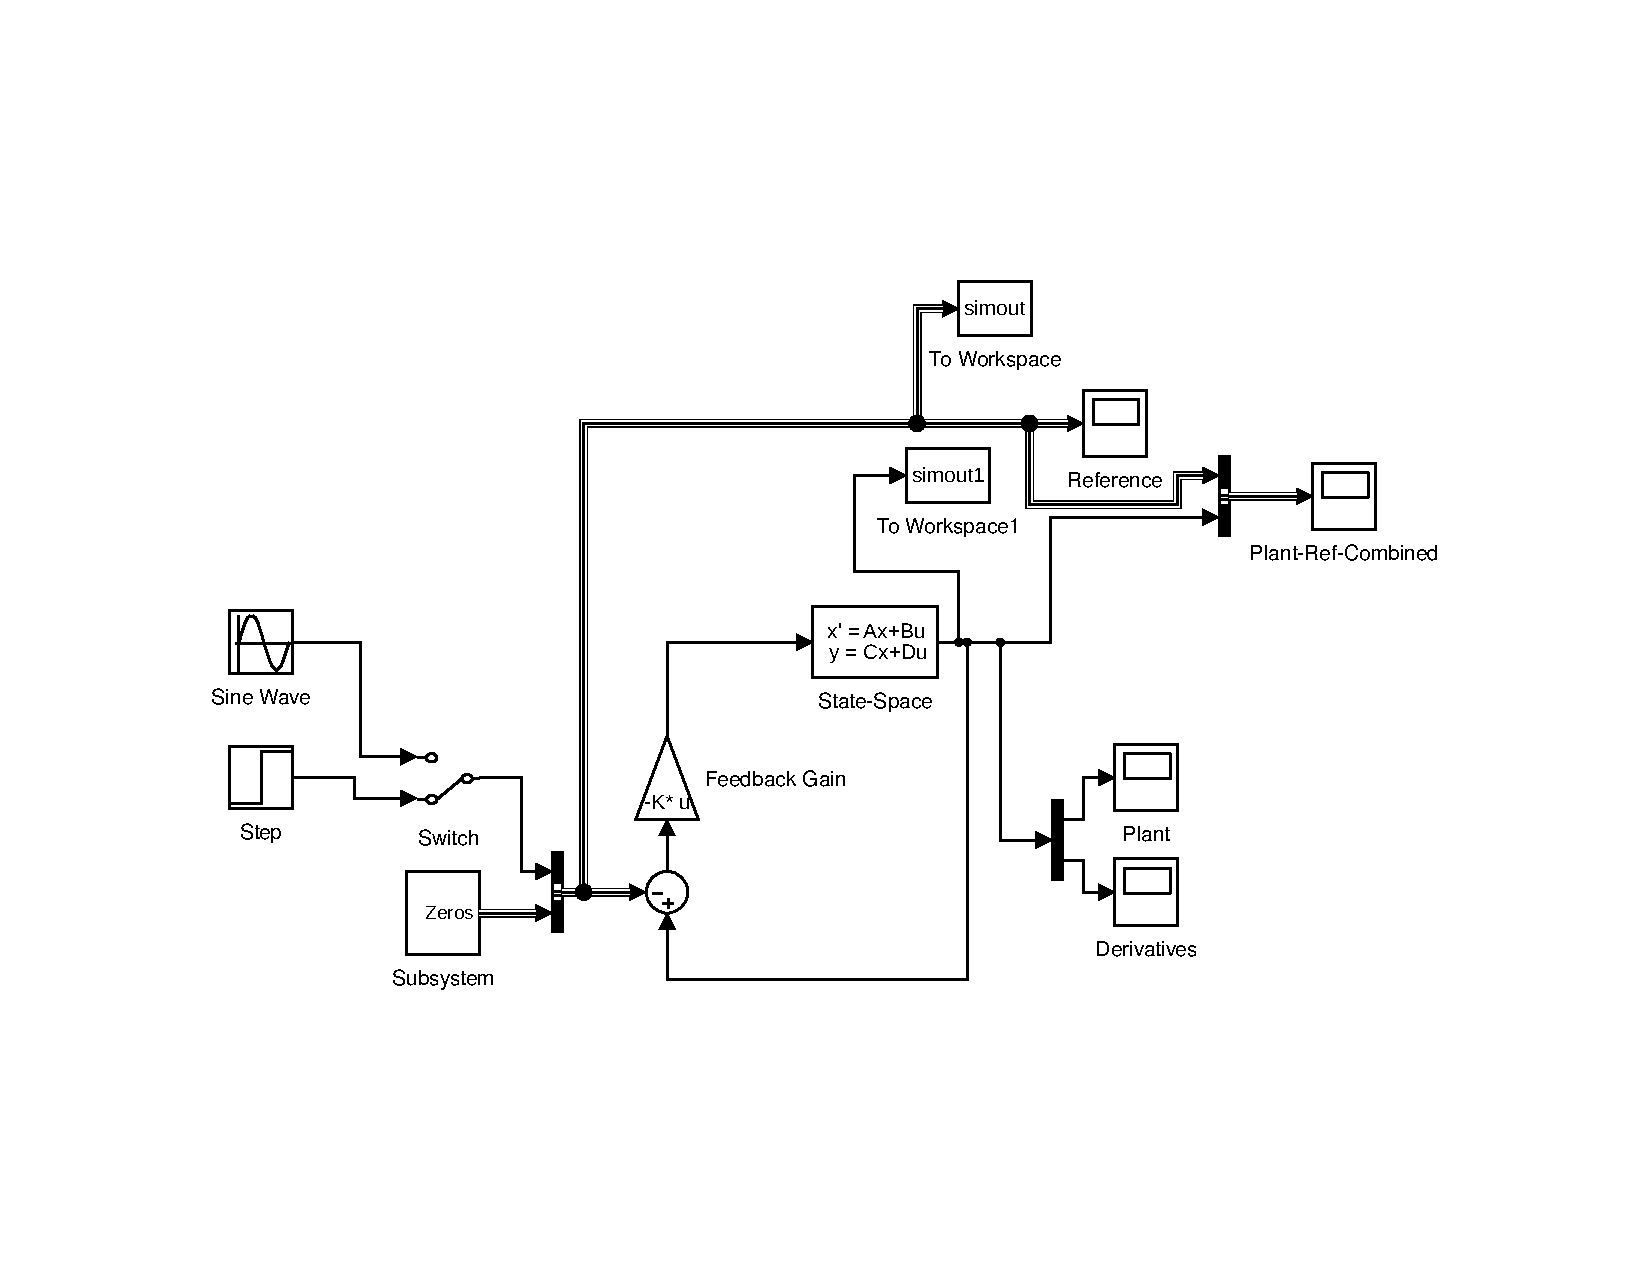
\includegraphics[scale=0.5]{images/simModelFullState.pdf}
\caption{The simulink Layout of our Simulation knowledge of all the states is assumed}
\label{fig:allStates}
\end{figure}
Figure~\ref{fig:allStates} shows our initial simulink diagram. The most important block in the control gain, that does the actual LQR-Control. The state space block in the center contains the continuous time system we showed in the previous section. In the left we have a selector that we use to choose between either a step or a sinusodial input. Below it we use a block of constant zeros to full up remaining entries of the input vector. 
As stated earlier we are using LQR-Control in this project. To compute the gain matrix for an LQR-Controller determines an state-feedback gain which minimizes the following cost function:
\begin{equation}
J = \int(\mathbf{x}^T Q \mathbf{x} + \mathbf{u}^T R \mathbf{u})dt.
\end{equation}
Initial but not optimal Q and R where given. \marginpar{Q = diag([350 1500 3 0.5]) for R = 10.} The $Q$ matrix gives weight to the different elements of the state vector. In our case hub position, arm position, angular hub and angular arm velocity. The R matrix, in our case a scalar makes the input more expensive. Our goals for tuning the controller are to achieve a satisfactory tracking for the hub angle $\theta$ without overshoot, while keeping the movement of the arm $\alpha$ as low as possible. At the same time we want to avoid actuator saturation. These are obviously conflicting objectives. So a good compromise is required. Figure~\ref{fig:stepResponse} shows the performance of the initially provided weighting parameters. From the tracking point of view the performance is not bad, however the input signal exceeds 5 Volts, which will lead to actuator saturation if applied to the real plant. We chose the following weighting matrix to fix this problem:
\begin{equation}
\begin{pmatrix}
500 &		&	&	\\
	&1000	&	&	\\
	&	&3	&	\\
	&	&	&10	\\
\end{pmatrix}
\end{equation}
With the input weight $R = 30$. We increased the weight on the inputs to prevent saturation. As a higher input weight will make high inputs more expensive we expected this to fix our saturation problem. Furthermore it turns out more effective to penalize the acceleration of $\dot{\alpha}$ in comparison to a high value for $\alpha$. This is the case because we know that the reference for $\alpha$ will always be zero. Putting a higher weight on arm-acceleration prevents the arm from moving too fast away from its zero reference. In figure~{\ref{fig:stepResponse} on the right side we show the simulated behavior with our adapted weights, where the tracking remains comparably fast. 


\begin{figure}
%% This file was created by matlab2tikz v0.4.7 running on MATLAB 8.4.
% Copyright (c) 2008--2014, Nico Schlömer <nico.schloemer@gmail.com>
% All rights reserved.
% Minimal pgfplots version: 1.3
% 
% The latest updates can be retrieved from
%   http://www.mathworks.com/matlabcentral/fileexchange/22022-matlab2tikz
% where you can also make suggestions and rate matlab2tikz.
% 
\documentclass[tikz]{standalone}
\usepackage{pgfplots}
\usepackage{grffile}
\pgfplotsset{compat=newest}
\usetikzlibrary{plotmarks}
\usepackage{amsmath}

\begin{document}
%
% defining custom colors
\definecolor{mycolor1}{rgb}{0.00000,0.44700,0.74100}%
\definecolor{mycolor2}{rgb}{0.85000,0.32500,0.09800}%
\definecolor{mycolor3}{rgb}{0.92900,0.69400,0.12500}%
%
\begin{tikzpicture}

\begin{axis}[%
width=1.8in,
height=1in,
scale only axis,
separate axis lines,
every outer x axis line/.append style={white!15!black},
every x tick label/.append style={font=\color{white!15!black}},
xmin=0,
xmax=5,
every outer y axis line/.append style={white!15!black},
every y tick label/.append style={font=\color{white!15!black}},
ymin=-0.2,
ymax=0.8,
name=plot1,
%title style={font=\bfseries},
ylabel={plant, reference [rad]}
]
\addplot [color=mycolor1,solid,forget plot]
  table[row sep=crcr]{0	0\\
0.005	0\\
0.01	0\\
0.015	0\\
0.02	0\\
0.025	0\\
0.03	0\\
0.035	0\\
0.04	0\\
0.045	0\\
0.05	0\\
0.055	0\\
0.06	0\\
0.065	0\\
0.07	0\\
0.075	0\\
0.08	0\\
0.085	0\\
0.09	0\\
0.095	0\\
0.1	0\\
0.105	0\\
0.11	0\\
0.115	0\\
0.12	0\\
0.125	0\\
0.13	0\\
0.135	0\\
0.14	0\\
0.145	0\\
0.15	0\\
0.155	0\\
0.16	0\\
0.165	0\\
0.17	0\\
0.175	0\\
0.18	0\\
0.185	0\\
0.19	0\\
0.195	0\\
0.2	0\\
0.205	0\\
0.21	0\\
0.215	0\\
0.22	0\\
0.225	0\\
0.23	0\\
0.235	0\\
0.24	0\\
0.245	0\\
0.25	0\\
0.255	0\\
0.26	0\\
0.265	0\\
0.27	0\\
0.275	0\\
0.28	0\\
0.285	0\\
0.29	0\\
0.295	0\\
0.3	0\\
0.305	0\\
0.31	0\\
0.315	0\\
0.32	0\\
0.325	0\\
0.33	0\\
0.335	0\\
0.34	0\\
0.345	0\\
0.35	0\\
0.355	0\\
0.36	0\\
0.365	0\\
0.37	0\\
0.375	0\\
0.38	0\\
0.385	0\\
0.39	0\\
0.395	0\\
0.4	0\\
0.405	0\\
0.41	0\\
0.415	0\\
0.42	0\\
0.425	0\\
0.43	0\\
0.435	0\\
0.44	0\\
0.445	0\\
0.45	0\\
0.455	0\\
0.46	0\\
0.465	0\\
0.47	0\\
0.475	0\\
0.48	0\\
0.485	0\\
0.49	0\\
0.495	0\\
0.5	0\\
0.505	0\\
0.51	0\\
0.515	0\\
0.52	0\\
0.525	0\\
0.53	0\\
0.535	0\\
0.54	0\\
0.545	0\\
0.55	0\\
0.555	0\\
0.56	0\\
0.565	0\\
0.57	0\\
0.575	0\\
0.58	0\\
0.585	0\\
0.59	0\\
0.595	0\\
0.6	0\\
0.605	0\\
0.61	0\\
0.615	0\\
0.62	0\\
0.625	0\\
0.63	0\\
0.635	0\\
0.64	0\\
0.645	0\\
0.65	0\\
0.655	0\\
0.66	0\\
0.665	0\\
0.67	0\\
0.675	0\\
0.68	0\\
0.685	0\\
0.69	0\\
0.695	0\\
0.7	0\\
0.705	0\\
0.71	0\\
0.715	0\\
0.72	0\\
0.725	0\\
0.73	0\\
0.735	0\\
0.74	0\\
0.745	0\\
0.75	0\\
0.755	0\\
0.76	0\\
0.765	0\\
0.77	0\\
0.775	0\\
0.78	0\\
0.785	0\\
0.79	0\\
0.795	0\\
0.8	0\\
0.805	0\\
0.81	0\\
0.815	0\\
0.82	0\\
0.825	0\\
0.83	0\\
0.835	0\\
0.84	0\\
0.845	0\\
0.85	0\\
0.855	0\\
0.86	0\\
0.865	0\\
0.87	0\\
0.875	0\\
0.88	0\\
0.885	0\\
0.89	0\\
0.895	0\\
0.9	0\\
0.905	0\\
0.91	0\\
0.915	0\\
0.92	0\\
0.925	0\\
0.93	0\\
0.935	0\\
0.94	0\\
0.945	0\\
0.95	0\\
0.955	0\\
0.96	0\\
0.965	0\\
0.97	0\\
0.975	0\\
0.98	0\\
0.985	0\\
0.99	0\\
0.995	0\\
1	0\\
1.005	0.00523203624393392\\
1.01	0.018186605839208\\
1.015	0.0352342868591856\\
1.02	0.0539958675836227\\
1.025	0.0729538401874592\\
1.03	0.0911814985665003\\
1.035	0.108154164435518\\
1.04	0.123617771729083\\
1.045	0.137497513309732\\
1.05	0.149834471777402\\
1.055	0.160741798933166\\
1.06	0.170374551688914\\
1.065	0.178909067882093\\
1.07	0.18652900528233\\
1.075	0.193416032833595\\
1.08	0.199743767790938\\
1.085	0.205673974718829\\
1.09	0.211354337351883\\
1.095	0.216917320495604\\
1.1	0.222479783283137\\
1.105	0.228143105925134\\
1.11	0.233993662662367\\
1.115	0.240103523077566\\
1.12	0.24653129861244\\
1.125	0.253323075513464\\
1.13	0.260513392599091\\
1.135	0.268126234367861\\
1.14	0.276176018563894\\
1.145	0.284668563439095\\
1.15	0.293602024337562\\
1.155	0.302967792391718\\
1.16	0.312751350421486\\
1.165	0.322933082818445\\
1.17	0.333489037452368\\
1.175	0.344391638580611\\
1.18	0.355610350457881\\
1.185	0.367112291895478\\
1.19	0.378862802447752\\
1.195	0.39082596123959\\
1.2	0.402965059713482\\
1.205	0.415243029783715\\
1.21	0.427622829049477\\
1.215	0.440067784846418\\
1.22	0.452541899013558\\
1.225	0.465010115324052\\
1.23	0.477438551577801\\
1.235	0.489794698384265\\
1.24	0.502047586677305\\
1.245	0.514167926002721\\
1.25	0.526128215604857\\
1.255	0.537902830313022\\
1.26	0.54946808319269\\
1.265	0.560802266881934\\
1.27	0.571885675481361\\
1.275	0.582700608807132\\
1.28	0.593231360752331\\
1.285	0.603464193433073\\
1.29	0.613387298723041\\
1.295	0.6229907487045\\
1.3	0.632266436485938\\
1.305	0.641208008757046\\
1.31	0.649810791371382\\
1.315	0.658071709166338\\
1.32	0.665989201149497\\
1.325	0.673563132100536\\
1.33	0.680794701559025\\
1.335	0.687686351091074\\
1.34	0.694241670652191\\
1.345	0.700465304790197\\
1.35	0.706362859360872\\
1.355	0.711940809360391\\
1.36	0.717206408412709\\
1.365	0.722167600387061\\
1.37	0.726832933560775\\
1.375	0.731211477685625\\
1.38	0.735312744262281\\
1.385	0.739146610276779\\
1.39	0.74272324560561\\
1.395	0.746053044251857\\
1.4	0.749146559533802\\
1.405	0.752014443309568\\
1.41	0.754667389286558\\
1.415	0.757116080432633\\
1.42	0.759371140477116\\
1.425	0.76144308946361\\
1.43	0.763342303293271\\
1.435	0.765078977176455\\
1.44	0.766663092892383\\
1.445	0.768104389740616\\
1.45	0.769412339054492\\
1.455	0.770596122135182\\
1.46	0.771664611455526\\
1.465	0.772626354975165\\
1.47	0.773489563402598\\
1.475	0.774262100235515\\
1.48	0.774951474407985\\
1.485	0.77556483537163\\
1.49	0.776108970437781\\
1.495	0.776590304208553\\
1.5	0.777014899926774\\
1.505	0.777388462577599\\
1.51	0.777716343578334\\
1.515	0.77800354689743\\
1.52	0.77825473644863\\
1.525	0.778474244611791\\
1.53	0.77866608173794\\
1.535	0.778833946502436\\
1.54	0.778981236976806\\
1.545	0.779111062296642\\
1.55	0.779226254810009\\
1.555	0.779329382597903\\
1.56	0.779422762265478\\
1.565	0.779508471909898\\
1.57	0.779588364177768\\
1.575	0.779664079332135\\
1.58	0.77973705825588\\
1.585	0.779808555325088\\
1.59	0.779879651092488\\
1.595	0.779951264727374\\
1.6	0.780024166164523\\
1.605	0.780098987920441\\
1.61	0.780176236540865\\
1.615	0.780256303648721\\
1.62	0.780339476566789\\
1.625	0.780425948494016\\
1.63	0.780515828218898\\
1.635	0.780609149357447\\
1.64	0.780705879107156\\
1.645	0.780805926511913\\
1.65	0.780909150236081\\
1.655	0.781015365848986\\
1.66	0.781124352623757\\
1.665	0.781235859856914\\
1.67	0.781349612717323\\
1.675	0.78146531763506\\
1.68	0.781582667242469\\
1.685	0.781701344881166\\
1.69	0.781821028690034\\
1.695	0.781941395290304\\
1.7	0.782062123084725\\
1.705	0.78218289518849\\
1.71	0.782303402010148\\
1.715	0.782423343501092\\
1.72	0.782542431092445\\
1.725	0.782660389338271\\
1.73	0.782776957284001\\
1.735	0.782891889578862\\
1.74	0.783004957350819\\
1.745	0.783115948862261\\
1.75	0.78322466996424\\
1.755	0.783330944366603\\
1.76	0.783434613740823\\
1.765	0.783535537671783\\
1.77	0.783633593474079\\
1.775	0.783728675887817\\
1.78	0.783820696668139\\
1.785	0.783909584082021\\
1.79	0.783995282325145\\
1.795	0.784077750870941\\
1.8	0.784156963763106\\
1.805	0.784232908862202\\
1.81	0.784305587056185\\
1.815	0.784375011443996\\
1.82	0.78444120650061\\
1.825	0.784504207231271\\
1.83	0.784564058321931\\
1.835	0.784620813292271\\
1.84	0.784674533657029\\
1.845	0.784725288100765\\
1.85	0.784773151670588\\
1.855	0.784818204990824\\
1.86	0.784860533503076\\
1.865	0.784900226734607\\
1.87	0.784937377597525\\
1.875	0.784972081720795\\
1.88	0.785004436816686\\
1.885	0.785034542082893\\
1.89	0.785062497641197\\
1.895	0.785088404013206\\
1.9	0.785112361633437\\
1.905	0.785134470399696\\
1.91	0.785154829260488\\
1.915	0.785173535838968\\
1.92	0.785190686092727\\
1.925	0.785206374008561\\
1.93	0.78522069133119\\
1.935	0.785233727324798\\
1.94	0.785245568566103\\
1.945	0.78525629876764\\
1.95	0.785265998629796\\
1.955	0.785274745720137\\
1.96	0.785282614378482\\
1.965	0.785289675646162\\
1.97	0.7852959972179\\
1.975	0.785301643414729\\
1.98	0.785306675176356\\
1.985	0.785311150071437\\
1.99	0.785315122324208\\
1.995	0.785318642855978\\
2	0.785321759340015\\
2.005	0.78532451626841\\
2.01	0.785326955029534\\
2.015	0.785329113994788\\
2.02	0.785331028613374\\
2.025	0.78533273151389\\
2.03	0.78533425261161\\
2.035	0.785335619220382\\
2.04	0.785336856168125\\
2.045	0.785337985914983\\
2.05	0.785339028673272\\
2.055	0.785340002528383\\
2.06	0.785340923559915\\
2.065	0.78534180596234\\
2.07	0.785342662164581\\
2.075	0.785343502947937\\
2.08	0.785344337561857\\
2.085	0.785345173837105\\
2.09	0.785346018295934\\
2.095	0.785346876258912\\
2.1	0.78534775194812\\
2.105	0.785348648586466\\
2.11	0.785349568492922\\
2.115	0.785350513173509\\
2.12	0.785351483407917\\
2.125	0.785352479331678\\
2.13	0.785353500513823\\
2.135	0.785354546030014\\
2.14	0.785355614531151\\
2.145	0.785356704307484\\
2.15	0.78535781334829\\
2.155	0.78535893939718\\
2.16	0.785360080003136\\
2.165	0.785361232567392\\
2.17	0.785362394386272\\
2.175	0.785363562690125\\
2.18	0.785364734678508\\
2.185	0.785365907551767\\
2.19	0.785367078539178\\
2.195	0.785368244923816\\
2.2	0.785369404064316\\
2.205	0.785370553413718\\
2.21	0.785371690535539\\
2.215	0.785372813117282\\
2.22	0.785373918981522\\
2.225	0.785375006094763\\
2.23	0.785376072574228\\
2.235	0.785377116692744\\
2.24	0.785378136881882\\
2.245	0.785379131733512\\
2.25	0.785380099999932\\
2.255	0.785381040592688\\
2.26	0.785381952580263\\
2.265	0.785382835184734\\
2.27	0.785383687777546\\
2.275	0.785384509874504\\
2.28	0.78538530113012\\
2.285	0.785386061331391\\
2.29	0.785386790391139\\
2.295	0.785387488340977\\
2.3	0.785388155324007\\
2.305	0.785388791587321\\
2.31	0.785389397474376\\
2.315	0.785389973417313\\
2.32	0.785390519929282\\
2.325	0.785391037596823\\
2.33	0.785391527072348\\
2.335	0.785391989066783\\
2.34	0.785392424342393\\
2.345	0.78539283370582\\
2.35	0.785393218001386\\
2.355	0.785393578104653\\
2.36	0.785393914916288\\
2.365	0.785394229356231\\
2.37	0.785394522358185\\
2.375	0.785394794864438\\
2.38	0.785395047821019\\
2.385	0.785395282173194\\
2.39	0.785395498861305\\
2.395	0.785395698816941\\
2.4	0.78539588295945\\
2.405	0.785396052192773\\
2.41	0.785396207402604\\
2.415	0.785396349453858\\
2.42	0.785396479188447\\
2.425	0.785396597423339\\
2.43	0.785396704948898\\
2.435	0.785396802527497\\
2.44	0.785396890892372\\
2.445	0.785396970746724\\
2.45	0.785397042763039\\
2.455	0.785397107582619\\
2.46	0.785397165815315\\
2.465	0.78539721803943\\
2.47	0.785397264801799\\
2.475	0.785397306618015\\
2.48	0.7853973439728\\
2.485	0.785397377320492\\
2.49	0.785397407085656\\
2.495	0.785397433663786\\
2.5	0.785397457422097\\
2.505	0.785397478700395\\
2.51	0.785397497812007\\
2.515	0.785397515044773\\
2.52	0.785397530662071\\
2.525	0.785397544903887\\
2.53	0.785397557987906\\
2.535	0.785397570110621\\
2.54	0.785397581448456\\
2.545	0.785397592158884\\
2.55	0.785397602381552\\
2.555	0.785397612239389\\
2.56	0.785397621839705\\
2.565	0.785397631275267\\
2.57	0.785397640625354\\
2.575	0.785397649956785\\
2.58	0.785397659324914\\
2.585	0.7853976687746\\
2.59	0.785397678341126\\
2.595	0.785397688051099\\
2.6	0.785397697923299\\
2.605	0.785397707969492\\
2.61	0.785397718195201\\
2.615	0.785397728600433\\
2.62	0.785397739180374\\
2.625	0.78539774992603\\
2.63	0.785397760824829\\
2.635	0.785397771861194\\
2.64	0.785397783017055\\
2.645	0.78539779427234\\
2.65	0.785397805605418\\
2.655	0.785397816993503\\
2.66	0.785397828413028\\
2.665	0.785397839839982\\
2.67	0.785397851250207\\
2.675	0.785397862619673\\
2.68	0.785397873924715\\
2.685	0.785397885142243\\
2.69	0.785397896249929\\
2.695	0.785397907226357\\
2.7	0.785397918051163\\
2.705	0.785397928705142\\
2.71	0.785397939170336\\
2.715	0.785397949430106\\
2.72	0.785397959469181\\
2.725	0.785397969273698\\
2.73	0.785397978831216\\
2.735	0.785397988130727\\
2.74	0.78539799716265\\
2.745	0.785398005918811\\
2.75	0.78539801439242\\
2.755	0.785398022578034\\
2.76	0.785398030471516\\
2.765	0.785398038069983\\
2.77	0.785398045371758\\
2.775	0.785398052376303\\
2.78	0.785398059084163\\
2.785	0.785398065496899\\
2.79	0.78539807161702\\
2.795	0.785398077447913\\
2.8	0.78539808299378\\
2.805	0.78539808825956\\
2.81	0.785398093250866\\
2.815	0.785398097973915\\
2.82	0.78539810243546\\
2.825	0.785398106642725\\
2.83	0.785398110603344\\
2.835	0.785398114325294\\
2.84	0.785398117816842\\
2.845	0.785398121086484\\
2.85	0.785398124142895\\
2.855	0.785398126994876\\
2.86	0.785398129651306\\
2.865	0.785398132121101\\
2.87	0.785398134413167\\
2.875	0.785398136536364\\
2.88	0.785398138499473\\
2.885	0.785398140311161\\
2.89	0.785398141979949\\
2.895	0.785398143514191\\
2.9	0.785398144922048\\
2.905	0.785398146211468\\
2.91	0.785398147390164\\
2.915	0.785398148465604\\
2.92	0.785398149444996\\
2.925	0.785398150335274\\
2.93	0.785398151143095\\
2.935	0.785398151874828\\
2.94	0.785398152536551\\
2.945	0.785398153134051\\
2.95	0.785398153672817\\
2.955	0.785398154158047\\
2.96	0.785398154594644\\
2.965	0.785398154987226\\
2.97	0.785398155340123\\
2.975	0.785398155657388\\
2.98	0.785398155942801\\
2.985	0.785398156199878\\
2.99	0.785398156431877\\
2.995	0.785398156641805\\
3	0.785398156832434\\
3.005	0.785398157006303\\
3.01	0.78539815716573\\
3.015	0.785398157312826\\
3.02	0.7853981574495\\
3.025	0.785398157577471\\
3.03	0.78539815769828\\
3.035	0.785398157813301\\
3.04	0.785398157923745\\
3.045	0.785398158030681\\
3.05	0.785398158135034\\
3.055	0.785398158237605\\
3.06	0.785398158339074\\
3.065	0.785398158440012\\
3.07	0.785398158540892\\
3.075	0.785398158642092\\
3.08	0.785398158743908\\
3.085	0.785398158846562\\
3.09	0.785398158950206\\
3.095	0.785398159054932\\
3.1	0.785398159160781\\
3.105	0.785398159267743\\
3.11	0.78539815937577\\
3.115	0.785398159484776\\
3.12	0.785398159594648\\
3.125	0.785398159705247\\
3.13	0.78539815981641\\
3.135	0.785398159927963\\
3.14	0.785398160039717\\
3.145	0.785398160151473\\
3.15	0.785398160263029\\
3.155	0.785398160374178\\
3.16	0.785398160484713\\
3.165	0.785398160594431\\
3.17	0.785398160703132\\
3.175	0.785398160810621\\
3.18	0.785398160916711\\
3.185	0.785398161021225\\
3.19	0.785398161123993\\
3.195	0.78539816122486\\
3.2	0.785398161323678\\
3.205	0.785398161420315\\
3.21	0.785398161514647\\
3.215	0.785398161606566\\
3.22	0.785398161695977\\
3.225	0.785398161782794\\
3.23	0.785398161866948\\
3.235	0.785398161948379\\
3.24	0.785398162027042\\
3.245	0.785398162102901\\
3.25	0.785398162175934\\
3.255	0.785398162246127\\
3.26	0.785398162313479\\
3.265	0.785398162377998\\
3.27	0.7853981624397\\
3.275	0.785398162498611\\
3.28	0.785398162554765\\
3.285	0.785398162608202\\
3.29	0.785398162658971\\
3.295	0.785398162707125\\
3.3	0.785398162752723\\
3.305	0.785398162795831\\
3.31	0.785398162836516\\
3.315	0.785398162874852\\
3.32	0.785398162910913\\
3.325	0.785398162944777\\
3.33	0.785398162976526\\
3.335	0.785398163006241\\
3.34	0.785398163034005\\
3.345	0.785398163059902\\
3.35	0.785398163084015\\
3.355	0.78539816310643\\
3.36	0.785398163127229\\
3.365	0.785398163146496\\
3.37	0.785398163164312\\
3.375	0.785398163180758\\
3.38	0.785398163195912\\
3.385	0.785398163209851\\
3.39	0.785398163222652\\
3.395	0.785398163234386\\
3.4	0.785398163245124\\
3.405	0.785398163254934\\
3.41	0.785398163263882\\
3.415	0.785398163272031\\
3.42	0.785398163279442\\
3.425	0.785398163286172\\
3.43	0.785398163292275\\
3.435	0.785398163297805\\
3.44	0.78539816330281\\
3.445	0.785398163307338\\
3.45	0.785398163311431\\
3.455	0.785398163315132\\
3.46	0.785398163318479\\
3.465	0.785398163321509\\
3.47	0.785398163324254\\
3.475	0.785398163326747\\
3.48	0.785398163329016\\
3.485	0.785398163331087\\
3.49	0.785398163332986\\
3.495	0.785398163334735\\
3.5	0.785398163336353\\
3.505	0.78539816333786\\
3.51	0.785398163339273\\
3.515	0.785398163340606\\
3.52	0.785398163341873\\
3.525	0.785398163343086\\
3.53	0.785398163344255\\
3.535	0.78539816334539\\
3.54	0.785398163346499\\
3.545	0.785398163347589\\
3.55	0.785398163348665\\
3.555	0.785398163349732\\
3.56	0.785398163350795\\
3.565	0.785398163351857\\
3.57	0.785398163352919\\
3.575	0.785398163353985\\
3.58	0.785398163355055\\
3.585	0.78539816335613\\
3.59	0.785398163357211\\
3.595	0.785398163358296\\
3.6	0.785398163359386\\
3.605	0.785398163360481\\
3.61	0.785398163361578\\
3.615	0.785398163362676\\
3.62	0.785398163363775\\
3.625	0.785398163364873\\
3.63	0.785398163365968\\
3.635	0.785398163367058\\
3.64	0.785398163368142\\
3.645	0.785398163369219\\
3.65	0.785398163370285\\
3.655	0.785398163371339\\
3.66	0.785398163372381\\
3.665	0.785398163373408\\
3.67	0.785398163374418\\
3.675	0.78539816337541\\
3.68	0.785398163376384\\
3.685	0.785398163377337\\
3.69	0.785398163378268\\
3.695	0.785398163379176\\
3.7	0.785398163380061\\
3.705	0.785398163380922\\
3.71	0.785398163381757\\
3.715	0.785398163382567\\
3.72	0.78539816338335\\
3.725	0.785398163384107\\
3.73	0.785398163384836\\
3.735	0.785398163385539\\
3.74	0.785398163386214\\
3.745	0.785398163386863\\
3.75	0.785398163387484\\
3.755	0.785398163388078\\
3.76	0.785398163388645\\
3.765	0.785398163389186\\
3.77	0.785398163389702\\
3.775	0.785398163390191\\
3.78	0.785398163390656\\
3.785	0.785398163391097\\
3.79	0.785398163391513\\
3.795	0.785398163391907\\
3.8	0.785398163392278\\
3.805	0.785398163392628\\
3.81	0.785398163392956\\
3.815	0.785398163393265\\
3.82	0.785398163393554\\
3.825	0.785398163393824\\
3.83	0.785398163394077\\
3.835	0.785398163394312\\
3.84	0.785398163394531\\
3.845	0.785398163394735\\
3.85	0.785398163394924\\
3.855	0.785398163395099\\
3.86	0.785398163395261\\
3.865	0.785398163395411\\
3.87	0.785398163395548\\
3.875	0.785398163395675\\
3.88	0.785398163395792\\
3.885	0.785398163395899\\
3.89	0.785398163395997\\
3.895	0.785398163396087\\
3.9	0.785398163396169\\
3.905	0.785398163396244\\
3.91	0.785398163396312\\
3.915	0.785398163396374\\
3.92	0.785398163396431\\
3.925	0.785398163396482\\
3.93	0.785398163396529\\
3.935	0.785398163396571\\
3.94	0.78539816339661\\
3.945	0.785398163396645\\
3.95	0.785398163396676\\
3.955	0.785398163396705\\
3.96	0.785398163396732\\
3.965	0.785398163396756\\
3.97	0.785398163396778\\
3.975	0.785398163396799\\
3.98	0.785398163396818\\
3.985	0.785398163396835\\
3.99	0.785398163396852\\
3.995	0.785398163396867\\
4	0.785398163396881\\
4.005	0.785398163396895\\
4.01	0.785398163396908\\
4.015	0.785398163396921\\
4.02	0.785398163396933\\
4.025	0.785398163396945\\
4.03	0.785398163396956\\
4.035	0.785398163396968\\
4.04	0.785398163396979\\
4.045	0.78539816339699\\
4.05	0.785398163397001\\
4.055	0.785398163397012\\
4.06	0.785398163397023\\
4.065	0.785398163397034\\
4.07	0.785398163397045\\
4.075	0.785398163397056\\
4.08	0.785398163397066\\
4.085	0.785398163397077\\
4.09	0.785398163397088\\
4.095	0.785398163397099\\
4.1	0.78539816339711\\
4.105	0.785398163397121\\
4.11	0.785398163397132\\
4.115	0.785398163397142\\
4.12	0.785398163397153\\
4.125	0.785398163397164\\
4.13	0.785398163397174\\
4.135	0.785398163397184\\
4.14	0.785398163397195\\
4.145	0.785398163397205\\
4.15	0.785398163397215\\
4.155	0.785398163397225\\
4.16	0.785398163397234\\
4.165	0.785398163397244\\
4.17	0.785398163397253\\
4.175	0.785398163397262\\
4.18	0.785398163397271\\
4.185	0.785398163397279\\
4.19	0.785398163397288\\
4.195	0.785398163397296\\
4.2	0.785398163397303\\
4.205	0.785398163397311\\
4.21	0.785398163397318\\
4.215	0.785398163397325\\
4.22	0.785398163397332\\
4.225	0.785398163397339\\
4.23	0.785398163397345\\
4.235	0.785398163397351\\
4.24	0.785398163397357\\
4.245	0.785398163397362\\
4.25	0.785398163397367\\
4.255	0.785398163397372\\
4.26	0.785398163397377\\
4.265	0.785398163397381\\
4.27	0.785398163397386\\
4.275	0.78539816339739\\
4.28	0.785398163397393\\
4.285	0.785398163397397\\
4.29	0.7853981633974\\
4.295	0.785398163397404\\
4.3	0.785398163397407\\
4.305	0.785398163397409\\
4.31	0.785398163397412\\
4.315	0.785398163397415\\
4.32	0.785398163397417\\
4.325	0.785398163397419\\
4.33	0.785398163397421\\
4.335	0.785398163397423\\
4.34	0.785398163397425\\
4.345	0.785398163397426\\
4.35	0.785398163397428\\
4.355	0.785398163397429\\
4.36	0.78539816339743\\
4.365	0.785398163397431\\
4.37	0.785398163397432\\
4.375	0.785398163397433\\
4.38	0.785398163397434\\
4.385	0.785398163397435\\
4.39	0.785398163397436\\
4.395	0.785398163397437\\
4.4	0.785398163397437\\
4.405	0.785398163397438\\
4.41	0.785398163397438\\
4.415	0.785398163397439\\
4.42	0.785398163397439\\
4.425	0.78539816339744\\
4.43	0.78539816339744\\
4.435	0.78539816339744\\
4.44	0.785398163397441\\
4.445	0.785398163397441\\
4.45	0.785398163397441\\
4.455	0.785398163397441\\
4.46	0.785398163397442\\
4.465	0.785398163397442\\
4.47	0.785398163397442\\
4.475	0.785398163397442\\
4.48	0.785398163397442\\
4.485	0.785398163397443\\
4.49	0.785398163397443\\
4.495	0.785398163397443\\
4.5	0.785398163397443\\
4.505	0.785398163397443\\
4.51	0.785398163397443\\
4.515	0.785398163397443\\
4.52	0.785398163397443\\
4.525	0.785398163397443\\
4.53	0.785398163397444\\
4.535	0.785398163397444\\
4.54	0.785398163397444\\
4.545	0.785398163397444\\
4.55	0.785398163397444\\
4.555	0.785398163397444\\
4.56	0.785398163397444\\
4.565	0.785398163397444\\
4.57	0.785398163397444\\
4.575	0.785398163397445\\
4.58	0.785398163397445\\
4.585	0.785398163397445\\
4.59	0.785398163397445\\
4.595	0.785398163397445\\
4.6	0.785398163397445\\
4.605	0.785398163397445\\
4.61	0.785398163397445\\
4.615	0.785398163397445\\
4.62	0.785398163397446\\
4.625	0.785398163397446\\
4.63	0.785398163397446\\
4.635	0.785398163397446\\
4.64	0.785398163397446\\
4.645	0.785398163397446\\
4.65	0.785398163397446\\
4.655	0.785398163397446\\
4.66	0.785398163397446\\
4.665	0.785398163397447\\
4.67	0.785398163397447\\
4.675	0.785398163397447\\
4.68	0.785398163397447\\
4.685	0.785398163397447\\
4.69	0.785398163397447\\
4.695	0.785398163397447\\
4.7	0.785398163397447\\
4.705	0.785398163397447\\
4.71	0.785398163397448\\
4.715	0.785398163397448\\
4.72	0.785398163397448\\
4.725	0.785398163397448\\
4.73	0.785398163397448\\
4.735	0.785398163397448\\
4.74	0.785398163397448\\
4.745	0.785398163397448\\
4.75	0.785398163397448\\
4.755	0.785398163397448\\
4.76	0.785398163397448\\
4.765	0.785398163397448\\
4.77	0.785398163397448\\
4.775	0.785398163397448\\
4.78	0.785398163397448\\
4.785	0.785398163397448\\
4.79	0.785398163397448\\
4.795	0.785398163397448\\
4.8	0.785398163397448\\
4.805	0.785398163397448\\
4.81	0.785398163397448\\
4.815	0.785398163397448\\
4.82	0.785398163397448\\
4.825	0.785398163397448\\
4.83	0.785398163397448\\
4.835	0.785398163397448\\
4.84	0.785398163397448\\
4.845	0.785398163397448\\
4.85	0.785398163397448\\
4.855	0.785398163397448\\
4.86	0.785398163397448\\
4.865	0.785398163397448\\
4.87	0.785398163397448\\
4.875	0.785398163397448\\
4.88	0.785398163397448\\
4.885	0.785398163397448\\
4.89	0.785398163397448\\
4.895	0.785398163397448\\
4.9	0.785398163397448\\
4.905	0.785398163397448\\
4.91	0.785398163397448\\
4.915	0.785398163397448\\
4.92	0.785398163397448\\
4.925	0.785398163397448\\
4.93	0.785398163397448\\
4.935	0.785398163397448\\
4.94	0.785398163397448\\
4.945	0.785398163397448\\
4.95	0.785398163397448\\
4.955	0.785398163397448\\
4.96	0.785398163397448\\
4.965	0.785398163397448\\
4.97	0.785398163397448\\
4.975	0.785398163397448\\
4.98	0.785398163397448\\
4.985	0.785398163397448\\
4.99	0.785398163397448\\
4.995	0.785398163397448\\
5	0.785398163397448\\
};
\addplot [color=mycolor2,solid,forget plot]
  table[row sep=crcr]{0	0\\
0.005	0\\
0.01	0\\
0.015	0\\
0.02	0\\
0.025	0\\
0.03	0\\
0.035	0\\
0.04	0\\
0.045	0\\
0.05	0\\
0.055	0\\
0.06	0\\
0.065	0\\
0.07	0\\
0.075	0\\
0.08	0\\
0.085	0\\
0.09	0\\
0.095	0\\
0.1	0\\
0.105	0\\
0.11	0\\
0.115	0\\
0.12	0\\
0.125	0\\
0.13	0\\
0.135	0\\
0.14	0\\
0.145	0\\
0.15	0\\
0.155	0\\
0.16	0\\
0.165	0\\
0.17	0\\
0.175	0\\
0.18	0\\
0.185	0\\
0.19	0\\
0.195	0\\
0.2	0\\
0.205	0\\
0.21	0\\
0.215	0\\
0.22	0\\
0.225	0\\
0.23	0\\
0.235	0\\
0.24	0\\
0.245	0\\
0.25	0\\
0.255	0\\
0.26	0\\
0.265	0\\
0.27	0\\
0.275	0\\
0.28	0\\
0.285	0\\
0.29	0\\
0.295	0\\
0.3	0\\
0.305	0\\
0.31	0\\
0.315	0\\
0.32	0\\
0.325	0\\
0.33	0\\
0.335	0\\
0.34	0\\
0.345	0\\
0.35	0\\
0.355	0\\
0.36	0\\
0.365	0\\
0.37	0\\
0.375	0\\
0.38	0\\
0.385	0\\
0.39	0\\
0.395	0\\
0.4	0\\
0.405	0\\
0.41	0\\
0.415	0\\
0.42	0\\
0.425	0\\
0.43	0\\
0.435	0\\
0.44	0\\
0.445	0\\
0.45	0\\
0.455	0\\
0.46	0\\
0.465	0\\
0.47	0\\
0.475	0\\
0.48	0\\
0.485	0\\
0.49	0\\
0.495	0\\
0.5	0\\
0.505	0\\
0.51	0\\
0.515	0\\
0.52	0\\
0.525	0\\
0.53	0\\
0.535	0\\
0.54	0\\
0.545	0\\
0.55	0\\
0.555	0\\
0.56	0\\
0.565	0\\
0.57	0\\
0.575	0\\
0.58	0\\
0.585	0\\
0.59	0\\
0.595	0\\
0.6	0\\
0.605	0\\
0.61	0\\
0.615	0\\
0.62	0\\
0.625	0\\
0.63	0\\
0.635	0\\
0.64	0\\
0.645	0\\
0.65	0\\
0.655	0\\
0.66	0\\
0.665	0\\
0.67	0\\
0.675	0\\
0.68	0\\
0.685	0\\
0.69	0\\
0.695	0\\
0.7	0\\
0.705	0\\
0.71	0\\
0.715	0\\
0.72	0\\
0.725	0\\
0.73	0\\
0.735	0\\
0.74	0\\
0.745	0\\
0.75	0\\
0.755	0\\
0.76	0\\
0.765	0\\
0.77	0\\
0.775	0\\
0.78	0\\
0.785	0\\
0.79	0\\
0.795	0\\
0.8	0\\
0.805	0\\
0.81	0\\
0.815	0\\
0.82	0\\
0.825	0\\
0.83	0\\
0.835	0\\
0.84	0\\
0.845	0\\
0.85	0\\
0.855	0\\
0.86	0\\
0.865	0\\
0.87	0\\
0.875	0\\
0.88	0\\
0.885	0\\
0.89	0\\
0.895	0\\
0.9	0\\
0.905	0\\
0.91	0\\
0.915	0\\
0.92	0\\
0.925	0\\
0.93	0\\
0.935	0\\
0.94	0\\
0.945	0\\
0.95	0\\
0.955	0\\
0.96	0\\
0.965	0\\
0.97	0\\
0.975	0\\
0.98	0\\
0.985	0\\
0.99	0\\
0.995	0\\
1	0\\
1.005	-0.00522895785388764\\
1.01	-0.018140478443417\\
1.015	-0.0350192359012344\\
1.02	-0.0533723828618899\\
1.025	-0.0715582452015607\\
1.03	-0.0885267561879355\\
1.035	-0.103637942408965\\
1.04	-0.116534941998379\\
1.045	-0.127055133947732\\
1.05	-0.13516791251939\\
1.055	-0.140931099966631\\
1.06	-0.144460405602637\\
1.065	-0.145908025051329\\
1.07	-0.145447650376318\\
1.075	-0.143263983380385\\
1.08	-0.139545417965598\\
1.085	-0.134478957925612\\
1.09	-0.128246716180759\\
1.095	-0.121023536753933\\
1.1	-0.112975417194006\\
1.105	-0.104258504464883\\
1.11	-0.0950185039444863\\
1.115	-0.085390387782719\\
1.12	-0.075498321498049\\
1.125	-0.065455750569575\\
1.13	-0.05536560485087\\
1.135	-0.0453205899492992\\
1.14	-0.0354035427141649\\
1.145	-0.0256878336598002\\
1.15	-0.0162378032135887\\
1.155	-0.00710922161080584\\
1.16	0.00165023560250704\\
1.165	0.010000502913985\\
1.17	0.0179086362997285\\
1.175	0.0253483251363851\\
1.18	0.0322994081977014\\
1.185	0.0387473967836846\\
1.19	0.0446830075534548\\
1.195	0.050101707230963\\
1.2	0.0550032710072106\\
1.205	0.0593913561604853\\
1.21	0.0632730921482778\\
1.215	0.0666586881846732\\
1.22	0.0695610591005942\\
1.225	0.0719954700881671\\
1.23	0.0739792007523578\\
1.235	0.0755312287312077\\
1.24	0.0766719329991639\\
1.245	0.0774228168351487\\
1.25	0.077806250317273\\
1.255	0.0778452320987489\\
1.26	0.0775631701239369\\
1.265	0.0769836808589477\\
1.27	0.0761304065372328\\
1.275	0.0750268498565632\\
1.28	0.0736962255091572\\
1.285	0.0721613278809166\\
1.29	0.0704444142182274\\
1.295	0.0685671025310246\\
1.3	0.0665502834782807\\
1.305	0.0644140454662276\\
1.31	0.0621776121799352\\
1.315	0.0598592917648495\\
1.32	0.0574764368760328\\
1.325	0.0550454148186787\\
1.33	0.0525815870135168\\
1.335	0.050099297034544\\
1.34	0.0476118664836674\\
1.345	0.0451315979869408\\
1.35	0.0426697846196868\\
1.355	0.040236725092595\\
1.36	0.0378417440574819\\
1.365	0.0354932169194905\\
1.37	0.0331985985717686\\
1.375	0.0309644554988204\\
1.38	0.0287965007254971\\
1.385	0.0266996311197464\\
1.39	0.024677966588538\\
1.395	0.0227348907376277\\
1.4	0.0208730925968228\\
1.405	0.0190946090430017\\
1.41	0.0174008675831654\\
1.415	0.0157927291891357\\
1.42	0.0142705309040324\\
1.425	0.0128341279682704\\
1.43	0.0114829352394329\\
1.435	0.0102159677059116\\
1.44	0.00903187991861981\\
1.445	0.00792900418831761\\
1.45	0.00690538741811721\\
1.455	0.00595882646152252\\
1.46	0.00508690191590359\\
1.465	0.00428701027958973\\
1.47	0.00355639441780429\\
1.475	0.00289217229845534\\
1.48	0.00229136397336926\\
1.485	0.00175091679392058\\
1.49	0.00126772886220925\\
1.495	0.000838670729990192\\
1.5	0.000460605367513933\\
1.505	0.000130406433325272\\
1.51	-0.000155025116062033\\
1.515	-0.000398746030802024\\
1.52	-0.000603757334882442\\
1.525	-0.000772992398947669\\
1.53	-0.000909306457643734\\
1.535	-0.00101546750686727\\
1.54	-0.00109414851354394\\
1.545	-0.00114792086848412\\
1.55	-0.0011792490114134\\
1.555	-0.00119048615640405\\
1.56	-0.00118387104559331\\
1.565	-0.00116152565921731\\
1.57	-0.00112545381057102\\
1.575	-0.0010775405554796\\
1.58	-0.00101955234719334\\
1.585	-0.000953137869255918\\
1.59	-0.000879829480804382\\
1.595	-0.000801045210903526\\
1.6	-0.000718091240860391\\
1.605	-0.000632164815974939\\
1.61	-0.000544357530828262\\
1.615	-0.000455658934961978\\
1.62	-0.000366960408633781\\
1.625	-0.000279059261220454\\
1.63	-0.000192663007756881\\
1.635	-0.00010839378202775\\
1.64	-2.67928475473982e-05\\
1.645	5.16748293437829e-05\\
1.65	0.00012661597718731\\
1.655	0.000197704418044603\\
1.66	0.000264676494463935\\
1.665	0.000327326549526926\\
1.67	0.000385502482165339\\
1.675	0.000439101397474669\\
1.68	0.000488065369389493\\
1.685	0.000532377330831662\\
1.69	0.000572057104300409\\
1.695	0.000607157583846495\\
1.7	0.000637761077462436\\
1.705	0.000663975817129083\\
1.71	0.000685932642085354\\
1.715	0.000703781859332588\\
1.72	0.00071769028394636\\
1.725	0.000727838460445189\\
1.73	0.000734418065254711\\
1.735	0.000737629489205171\\
1.74	0.000737679598005856\\
1.745	0.00073477966774909\\
1.75	0.000729143491704521\\
1.755	0.000720985653967529\\
1.76	0.000710519964919358\\
1.765	0.000697958052936402\\
1.77	0.000683508106347346\\
1.775	0.000667373759274831\\
1.78	0.000649753114708248\\
1.785	0.000630837897931253\\
1.79	0.000610812733267104\\
1.795	0.00058985453700194\\
1.8	0.000568132019296366\\
1.805	0.000545805287894259\\
1.81	0.000523025546480496\\
1.815	0.000499934880621796\\
1.82	0.000476666124342988\\
1.825	0.000453342800540877\\
1.83	0.000430079128615461\\
1.835	0.000406980092900161\\
1.84	0.000384141565695272\\
1.845	0.000361650478948966\\
1.85	0.000339585038884632\\
1.855	0.00031801497813937\\
1.86	0.000297001840253286\\
1.865	0.000276599291630453\\
1.87	0.000256853456377559\\
1.875	0.000237803269713471\\
1.88	0.000219480845929935\\
1.885	0.000201911857169036\\
1.89	0.000185115919564872\\
1.895	0.000169106983574085\\
1.9	0.000153893725590889\\
1.905	0.000139479938206159\\
1.91	0.000125864916725852\\
1.915	0.000113043839810828\\
1.92	0.000101008142337247\\
1.925	8.97458788036334e-05\\
1.93	7.92420758268851e-05\\
1.935	6.94790724747008e-05\\
1.94	6.04368473758028e-05\\
1.945	5.20933317317828e-05\\
1.95	4.44247075253877e-05\\
1.955	3.7405690379495e-05\\
1.96	3.10097966690984e-05\\
1.965	2.52095946253563e-05\\
1.97	1.99769392964517e-05\\
1.975	1.52831913448312e-05\\
1.98	1.10994197646934e-05\\
1.985	7.39658869765424e-06\\
1.99	4.14572860874558e-06\\
1.995	1.3180921596412e-06\\
2	-1.11470481829113e-06\\
2.005	-3.1805567914457e-06\\
2.01	-4.90675592337885e-06\\
2.015	-6.31989285642853e-06\\
2.02	-7.44577029192835e-06\\
2.025	-8.30932875829054e-06\\
2.03	-8.93458393548776e-06\\
2.035	-9.34457488959651e-06\\
2.04	-9.56132256163179e-06\\
2.045	-9.60579785045646e-06\\
2.05	-9.4978986296658e-06\\
2.055	-9.25643504258787e-06\\
2.06	-8.89912242750725e-06\\
2.065	-8.44258123651733e-06\\
2.07	-7.90234332565646e-06\\
2.075	-7.29286401081823e-06\\
2.08	-6.62753930300769e-06\\
2.085	-5.91872775751857e-06\\
2.09	-5.17777639421245e-06\\
2.095	-4.41505017000997e-06\\
2.1	-3.63996450968845e-06\\
2.105	-2.86102042684733e-06\\
2.11	-2.08584179324216e-06\\
2.115	-1.32121434136566e-06\\
2.12	-5.7312601198452e-07\\
2.125	1.53191714867308e-07\\
2.13	8.53221840343087e-07\\
2.135	1.52311952734204e-06\\
2.14	2.15966972405513e-06\\
2.145	2.76024498820731e-06\\
2.15	3.32276374522458e-06\\
2.155	3.84564918986133e-06\\
2.16	4.32778901798844e-06\\
2.165	4.76849615333599e-06\\
2.17	5.16747061305015e-06\\
2.175	5.52476263601e-06\\
2.18	5.84073717897642e-06\\
2.185	6.11603986784472e-06\\
2.19	6.35156447455492e-06\\
2.195	6.54842197458073e-06\\
2.2	6.70791122536605e-06\\
2.205	6.83149129259926e-06\\
2.21	6.92075543880555e-06\\
2.215	6.97740677735988e-06\\
2.22	7.00323558466241e-06\\
2.225	7.0000982538451e-06\\
2.23	6.96989786495623e-06\\
2.235	6.91456633907399e-06\\
2.24	6.83604813718026e-06\\
2.245	6.73628545884811e-06\\
2.25	6.61720489082249e-06\\
2.255	6.48070545135595e-06\\
2.26	6.32864797265922e-06\\
2.265	6.16284576099659e-06\\
2.27	5.98505647175259e-06\\
2.275	5.79697513517687e-06\\
2.28	5.60022826743396e-06\\
2.285	5.39636900100655e-06\\
2.29	5.18687316837395e-06\\
2.295	4.97313627317815e-06\\
2.3	4.75647128375359e-06\\
2.305	4.53810718490019e-06\\
2.31	4.31918822508032e-06\\
2.315	4.10077379778671e-06\\
2.32	3.88383889762658e-06\\
2.325	3.66927509366326e-06\\
2.33	3.45789196471968e-06\\
2.335	3.2504189436531e-06\\
2.34	3.04750752002368e-06\\
2.345	2.84973375308657e-06\\
2.35	2.65760104960526e-06\\
2.355	2.47154316358988e-06\\
2.36	2.29192737770028e-06\\
2.365	2.1190578286903e-06\\
2.37	1.95317894189257e-06\\
2.375	1.79447894234271e-06\\
2.38	1.64309341269872e-06\\
2.385	1.49910887061282e-06\\
2.39	1.3625663406543e-06\\
2.395	1.2334648982511e-06\\
2.4	1.11176516540796e-06\\
2.405	9.97392740155324e-07\\
2.41	8.90241543793707e-07\\
2.415	7.90177072009793e-07\\
2.42	6.97039537851557e-07\\
2.425	6.10646896356508e-07\\
2.43	5.30797742330643e-07\\
2.435	4.57274074375316e-07\\
2.44	3.89843919749738e-07\\
2.445	3.28263816042475e-07\\
2.45	2.72281146912053e-07\\
2.455	2.21636330335513e-07\\
2.46	1.76064858885086e-07\\
2.465	1.35299192535223e-07\\
2.47	9.90705053933882e-08\\
2.475	6.71102885443186e-08\\
2.48	3.91518119055222e-08\\
2.485	1.49314486181432e-08\\
2.49	-5.81013395706289e-09\\
2.495	-2.33269120983365e-08\\
2.5	-3.78665675034791e-08\\
2.505	-4.96696677260191e-08\\
2.51	-5.89689597377399e-08\\
2.515	-6.59887708824824e-08\\
2.52	-7.09445113317088e-08\\
2.525	-7.40422720548871e-08\\
2.53	-7.54785122646212e-08\\
2.535	-7.54398302863561e-08\\
2.54	-7.4102811829165e-08\\
2.545	-7.16339497006183e-08\\
2.55	-6.81896291012023e-08\\
2.555	-6.39161727593558e-08\\
2.56	-5.89499403161453e-08\\
2.565	-5.34174765344679e-08\\
2.57	-4.74357031013475e-08\\
2.575	-4.11121489921043e-08\\
2.58	-3.45452145788407e-08\\
2.585	-2.78244648970716e-08\\
2.59	-2.10309477160431e-08\\
2.595	-1.4237532300053e-08\\
2.6	-7.50926498928823e-09\\
2.605	-9.03737974868331e-10\\
2.61	5.52853210692388e-09\\
2.615	1.1743718897257e-08\\
2.62	1.77042972486609e-08\\
2.625	2.33786530225583e-08\\
2.63	2.87406941733195e-08\\
2.635	3.3769465317432e-08\\
2.64	3.84487677618899e-08\\
2.645	4.27667867596477e-08\\
2.65	4.67157275551998e-08\\
2.655	5.02914615874856e-08\\
2.66	5.3493184031976e-08\\
2.665	5.63230836911124e-08\\
2.67	5.87860260756139e-08\\
2.675	6.08892503611512e-08\\
2.68	6.26420807590315e-08\\
2.685	6.40556527050468e-08\\
2.69	6.51426541462239e-08\\
2.695	6.59170820849327e-08\\
2.7	6.63940144329667e-08\\
2.705	6.65893971338027e-08\\
2.71	6.6519846423106e-08\\
2.715	6.62024660135084e-08\\
2.72	6.5654678923354e-08\\
2.725	6.48940736047834e-08\\
2.73	6.39382639692457e-08\\
2.735	6.28047628644637e-08\\
2.74	6.15108685152921e-08\\
2.745	6.00735634072913e-08\\
2.75	5.85094250629805e-08\\
2.755	5.6834548139326e-08\\
2.76	5.50644772596443e-08\\
2.765	5.32141499813505e-08\\
2.77	5.12978492966095e-08\\
2.775	4.93291650577508e-08\\
2.78	4.73209637209748e-08\\
2.785	4.52853658108295e-08\\
2.79	4.32337305119993e-08\\
2.795	4.11766468069763e-08\\
2.8	3.91239305956458e-08\\
2.805	3.70846272461231e-08\\
2.81	3.50670190427641e-08\\
2.815	3.30786370167673e-08\\
2.82	3.11262766696005e-08\\
2.825	2.92160171181995e-08\\
2.83	2.73532432133716e-08\\
2.835	2.55426702073167e-08\\
2.84	2.37883705697049e-08\\
2.845	2.20938025768712e-08\\
2.85	2.04618403210806e-08\\
2.855	1.88948048140045e-08\\
2.86	1.7394495878502e-08\\
2.865	1.5962224546952e-08\\
2.87	1.45988457119668e-08\\
2.875	1.33047907935297e-08\\
2.88	1.20801002080626e-08\\
2.885	1.09244554507086e-08\\
2.89	9.83721061871489e-09\\
2.895	8.81742322372621e-09\\
2.9	7.86388415895427e-09\\
2.905	6.97514670787861e-09\\
2.91	6.1495544968345e-09\\
2.915	5.38526830771346e-09\\
2.92	4.68029168418638e-09\\
2.925	4.03249527626922e-09\\
2.93	3.43963988466784e-09\\
2.935	2.89939817742319e-09\\
2.94	2.40937505887428e-09\\
2.945	1.96712668429147e-09\\
2.95	1.57017812321039e-09\\
2.955	1.21603968225886e-09\\
2.96	9.02221905433151e-10\\
2.965	6.26249275298641e-10\\
2.97	3.85672646169937e-10\\
2.975	1.78080445878997e-10\\
2.98	1.10868694664663e-12\\
2.985	-1.47550169834926e-10\\
2.99	-2.70139451694594e-10\\
2.995	-3.68831559226322e-10\\
3	-4.45722248822245e-10\\
3.005	-5.02825859631029e-10\\
3.01	-5.42071429683966e-10\\
3.015	-5.65299646390764e-10\\
3.02	-5.74260575387966e-10\\
3.025	-5.70612112395608e-10\\
3.03	-5.55919104816481e-10\\
3.035	-5.31653086694298e-10\\
3.04	-4.99192575924255e-10\\
3.045	-4.59823882178359e-10\\
3.05	-4.14742373813907e-10\\
3.055	-3.65054156646033e-10\\
3.06	-3.11778117756115e-10\\
3.065	-2.55848289548452e-10\\
3.07	-1.9811649157249e-10\\
3.075	-1.39355209603136e-10\\
3.08	-8.02606731939758e-11\\
3.085	-2.1456096164391e-11\\
3.09	3.65049538195327e-11\\
3.095	9.31350876667626e-11\\
3.1	1.48009559041905e-10\\
3.105	2.00762688820943e-10\\
3.11	2.51084273354206e-10\\
3.115	2.98715997800916e-10\\
3.12	3.43447877256304e-10\\
3.125	3.8511474523507e-10\\
3.13	4.23592803822518e-10\\
3.135	4.58796250202409e-10\\
3.14	4.90673994288738e-10\\
3.145	5.19206479283942e-10\\
3.15	5.44402613070026e-10\\
3.155	5.66296818362613e-10\\
3.16	5.84946209319647e-10\\
3.165	6.00427898748172e-10\\
3.17	6.12836442514931e-10\\
3.175	6.22281421454907e-10\\
3.18	6.28885162248128e-10\\
3.185	6.32780600502036e-10\\
3.19	6.34109283466092e-10\\
3.195	6.33019512097582e-10\\
3.2	6.29664622303224e-10\\
3.205	6.24201400466502e-10\\
3.21	6.16788630686022e-10\\
3.215	6.0758577223146e-10\\
3.22	5.96751761427837e-10\\
3.225	5.84443932895698e-10\\
3.23	5.70817056627942e-10\\
3.235	5.5602248730254e-10\\
3.24	5.40207417552303e-10\\
3.245	5.23514231751098e-10\\
3.25	5.0607995491908e-10\\
3.255	4.88035789809394e-10\\
3.26	4.69506738312545e-10\\
3.265	4.50611300511834e-10\\
3.27	4.31461246460957e-10\\
3.275	4.12161455178169e-10\\
3.28	3.92809814416817e-10\\
3.285	3.73497176323264e-10\\
3.29	3.5430736567829e-10\\
3.295	3.35317234606728e-10\\
3.3	3.16596758541458e-10\\
3.305	2.98209169049558e-10\\
3.31	2.80211118604861e-10\\
3.315	2.62652874785779e-10\\
3.32	2.45578538424956e-10\\
3.325	2.29026282586879e-10\\
3.33	2.13028609331728e-10\\
3.335	1.97612620524597e-10\\
3.34	1.82800298792315e-10\\
3.345	1.68608796713646e-10\\
3.35	1.5505073145333e-10\\
3.355	1.421344823522e-10\\
3.36	1.29864489974158e-10\\
3.365	1.1824155341523e-10\\
3.37	1.07263124365824e-10\\
3.375	9.69235961356929e-11\\
3.38	8.72145872404823e-11\\
3.385	7.81252176704647e-11\\
3.39	6.96423762183634e-11\\
3.395	6.1750979327395e-11\\
3.4	5.44342189323546e-11\\
3.405	4.76737989864911e-11\\
3.41	4.14501612464515e-11\\
3.415	3.57426997108832e-11\\
3.42	3.05299621527244e-11\\
3.425	2.57898392403512e-11\\
3.43	2.14997424994742e-11\\
3.435	1.76367681386561e-11\\
3.44	1.41778494512533e-11\\
3.445	1.10998980588904e-11\\
3.45	8.37993166647678e-12\\
3.455	5.99519035408909e-12\\
3.46	3.92324262086473e-12\\
3.465	2.14207968639186e-12\\
3.47	6.30198169186021e-13\\
3.475	-6.33325955246856e-13\\
3.48	-1.66877328484e-12\\
3.485	-2.49572713356631e-12\\
3.49	-3.1330271999655e-12\\
3.495	-3.59873200663435e-12\\
3.5	-3.91008968994975e-12\\
3.505	-4.08351552988001e-12\\
3.51	-4.13457712905586e-12\\
3.515	-4.0779846125832e-12\\
3.52	-3.92758586173314e-12\\
3.525	-3.69636847434966e-12\\
3.53	-3.3964664540788e-12\\
3.535	-3.03917104703748e-12\\
3.54	-2.63494581147113e-12\\
3.545	-2.19344435686416e-12\\
3.55	-1.72353194341137e-12\\
3.555	-1.23330898006174e-12\\
3.56	-7.30136276139591e-13\\
3.565	-2.2066353234051e-13\\
3.57	2.89140895062847e-13\\
3.575	7.93958862746701e-13\\
3.58	1.28909157941178e-12\\
3.585	1.77042694760339e-12\\
3.59	2.23440595877681e-12\\
3.595	2.67799045508925e-12\\
3.6	3.09863038192014e-12\\
3.605	3.49423021475745e-12\\
3.61	3.86311599246715e-12\\
3.615	4.20400451949905e-12\\
3.62	4.51597206769577e-12\\
3.625	4.79842283179658e-12\\
3.63	5.05105998975531e-12\\
3.635	5.27385751025922e-12\\
3.64	5.46703259180723e-12\\
3.645	5.63101922614832e-12\\
3.65	5.76644341847705e-12\\
3.655	5.87409874454199e-12\\
3.66	5.95492405510073e-12\\
3.665	6.00998243581018e-12\\
3.67	6.04044006090194e-12\\
3.675	6.04754813859651e-12\\
3.68	6.03262624416613e-12\\
3.685	5.9970454770319e-12\\
3.69	5.94221340193307e-12\\
3.695	5.86956033323881e-12\\
3.7	5.78052694746489e-12\\
3.705	5.67655296200526e-12\\
3.71	5.55906697369739e-12\\
3.715	5.42947725846909e-12\\
3.72	5.28916365996485e-12\\
3.725	5.13947038439984e-12\\
3.73	4.98169983423251e-12\\
3.735	4.81710803499473e-12\\
3.74	4.64689917715267e-12\\
3.745	4.47222159768688e-12\\
3.75	4.29416544324529e-12\\
3.755	4.11376032721031e-12\\
3.76	3.93197394760308e-12\\
3.765	3.74971006038309e-12\\
3.77	3.56780795801674e-12\\
3.775	3.38704357639167e-12\\
3.78	3.20812972232974e-12\\
3.785	3.03171598184552e-12\\
3.79	2.85838939487934e-12\\
3.795	2.68867719405097e-12\\
3.8	2.52304786767299e-12\\
3.805	2.36191317255282e-12\\
3.81	2.20563040236419e-12\\
3.815	2.05450387267877e-12\\
3.82	1.90878871130608e-12\\
3.825	1.76869316899423e-12\\
3.83	1.6343803106346e-12\\
3.835	1.50597072228446e-12\\
3.84	1.38354593852697e-12\\
3.845	1.26715077384197e-12\\
3.85	1.15679596789728e-12\\
3.855	1.05246153271518e-12\\
3.86	9.54098477080684e-13\\
3.865	8.61631816149424e-13\\
3.87	7.74963407814298e-13\\
3.875	6.93974175286655e-13\\
3.88	6.18526508729938e-13\\
3.885	5.48466877962858e-13\\
3.89	4.83627671027946e-13\\
3.895	4.23829479370548e-13\\
3.9	3.68882622698405e-13\\
3.905	3.18589251156863e-13\\
3.91	2.72745374088302e-13\\
3.915	2.31141690271195e-13\\
3.92	1.93566397881314e-13\\
3.925	1.59806143021465e-13\\
3.93	1.29646814899665e-13\\
3.935	1.02874652092667e-13\\
3.94	7.92777442010841e-14\\
3.945	5.86474625297666e-14\\
3.95	4.07785579822951e-14\\
3.955	2.54705395956404e-14\\
3.96	1.25282145703761e-14\\
3.965	1.76261565570266e-15\\
3.97	-7.00888129719578e-15\\
3.975	-1.39626387907207e-14\\
3.98	-1.9267809578118e-14\\
3.985	-2.30861216836535e-14\\
3.99	-2.55714579025608e-14\\
3.995	-2.68700928262645e-14\\
4	-2.7120539520491e-14\\
4.005	-2.64533188846176e-14\\
4.01	-2.49905934937789e-14\\
4.015	-2.28466251877561e-14\\
4.02	-2.01278105998274e-14\\
4.025	-1.69327386535536e-14\\
4.03	-1.33527759601264e-14\\
4.035	-9.47241983613594e-15\\
4.04	-5.36939888692563e-15\\
4.045	-1.11402741390158e-15\\
4.05	3.23042285456604e-15\\
4.055	7.60679356450324e-15\\
4.06	1.19642046079169e-14\\
4.065	1.62573059419591e-14\\
4.07	2.04459162191778e-14\\
4.075	2.44953780350349e-14\\
4.08	2.83760191906881e-14\\
4.085	3.20627577715025e-14\\
4.09	3.55347914016905e-14\\
4.095	3.87753331184047e-14\\
4.1	4.17713706701483e-14\\
4.105	4.45134353649878e-14\\
4.11	4.69953726213072e-14\\
4.115	4.92133710925336e-14\\
4.12	5.11661145601722e-14\\
4.125	5.28546659427453e-14\\
4.13	5.42816967776553e-14\\
4.135	5.54523771778637e-14\\
4.14	5.63732631775705e-14\\
4.145	5.70517471725607e-14\\
4.15	5.74969664184637e-14\\
4.155	5.77195778486041e-14\\
4.16	5.77307950148091e-14\\
4.165	5.75425557277453e-14\\
4.17	5.7167432036638e-14\\
4.175	5.66178968325879e-14\\
4.18	5.59065229626553e-14\\
4.185	5.50460560981196e-14\\
4.19	5.40494089423112e-14\\
4.195	5.29296080075751e-14\\
4.2	5.16997134790599e-14\\
4.205	5.03719864962102e-14\\
4.21	4.89581784109027e-14\\
4.215	4.74702962862144e-14\\
4.22	4.59195950784171e-14\\
4.225	4.43167639194758e-14\\
4.23	4.26726355691099e-14\\
4.235	4.09971529612831e-14\\
4.24	3.92995494079827e-14\\
4.245	3.75890643747604e-14\\
4.25	3.58739240188556e-14\\
4.255	3.41615399057215e-14\\
4.26	3.24592457150741e-14\\
4.265	3.07740388683675e-14\\
4.27	2.91116746787934e-14\\
4.275	2.74769494180603e-14\\
4.28	2.58745014197982e-14\\
4.285	2.43086031966072e-14\\
4.29	2.27830352560887e-14\\
4.295	2.13017540213495e-14\\
4.3	1.9868470476369e-14\\
4.305	1.84857793056807e-14\\
4.31	1.7155344788689e-14\\
4.315	1.58787779072923e-14\\
4.32	1.46573561137108e-14\\
4.325	1.3491987409744e-14\\
4.33	1.23830741439381e-14\\
4.335	1.13305722369428e-14\\
4.34	1.03346569813627e-14\\
4.345	9.39543625581105e-15\\
4.35	8.51204176009238e-15\\
4.355	7.68292362000331e-15\\
4.36	6.90667033025892e-15\\
4.365	6.18182241545804e-15\\
4.37	5.50676757642041e-15\\
4.375	4.8804279163359e-15\\
4.38	4.30185478831569e-15\\
4.385	3.76937044124172e-15\\
4.39	3.28076245581477e-15\\
4.395	2.83416537782374e-15\\
4.4	2.42778108905402e-15\\
4.405	2.05983975752098e-15\\
4.41	1.72845702805103e-15\\
4.415	1.43168345933884e-15\\
4.42	1.16741851992906e-15\\
4.425	9.33496021809582e-16\\
4.43	7.28359566244508e-16\\
4.435	5.50034674906756e-16\\
4.44	3.96336466522e-16\\
4.445	2.65623346108762e-16\\
4.45	1.5655771087673e-16\\
4.455	6.72175892668509e-17\\
4.46	-4.6066013737396e-18\\
4.465	-6.06022945354683e-17\\
4.47	-1.02139628361384e-16\\
4.475	-1.30400397774212e-16\\
4.48	-1.46457744586021e-16\\
4.485	-1.52063123453658e-16\\
4.49	-1.49286187164279e-16\\
4.495	-1.39666529895706e-16\\
4.5	-1.2439628628348e-16\\
4.505	-1.04437424001503e-16\\
4.51	-8.05966618995799e-17\\
4.515	-5.3572954711945e-17\\
4.52	-2.39872773449194e-17\\
4.525	7.59895292105109e-18\\
4.53	4.0672691083597e-17\\
4.535	7.47626338298972e-17\\
4.54	1.09435402947052e-16\\
4.545	1.44293416218374e-16\\
4.55	1.78973720286117e-16\\
4.555	2.13147321868829e-16\\
4.56	2.46518724870864e-16\\
4.565	2.78825492804952e-16\\
4.57	3.0983772909169e-16\\
4.575	3.39357415582244e-16\\
4.58	3.67217580799385e-16\\
4.585	3.9328128960058e-16\\
4.59	4.17440458954699e-16\\
4.595	4.3961451272318e-16\\
4.6	4.59748893341366e-16\\
4.605	4.77813451154134e-16\\
4.61	4.93800733564089e-16\\
4.615	5.07724196560047e-16\\
4.62	5.19616360917134e-16\\
4.625	5.29526934606596e-16\\
4.63	5.37520921867845e-16\\
4.635	5.43676738079167e-16\\
4.64	5.48084348090039e-16\\
4.645	5.50843444101649e-16\\
4.65	5.52061677544381e-16\\
4.655	5.51852957734359e-16\\
4.66	5.50335828421585e-16\\
4.665	5.4763193169142e-16\\
4.67	5.43864567066744e-16\\
4.675	5.39157352094992e-16\\
4.68	5.33632989204941e-16\\
4.685	5.27412142192733e-16\\
4.69	5.20612424353846e-16\\
4.695	5.13347499024064e-16\\
4.7	5.05726292133423e-16\\
4.705	4.97852315316125e-16\\
4.71	4.89823097159157e-16\\
4.715	4.81729719313946e-16\\
4.72	4.73656453438987e-16\\
4.725	4.64941339335761e-16\\
4.73	4.54563403260372e-16\\
4.735	4.42004983590685e-16\\
4.74	4.2707500299382e-16\\
4.745	4.09792508868991e-16\\
4.75	3.90309612973634e-16\\
4.755	3.68860234397167e-16\\
4.76	3.45725787309869e-16\\
4.765	3.21212040060441e-16\\
4.77	2.9563338108539e-16\\
4.775	2.69302034908601e-16\\
4.78	2.4252062268663e-16\\
4.785	2.15577015547111e-16\\
4.79	1.88740789126344e-16\\
4.795	1.62260821831364e-16\\
4.8	1.36363731464742e-16\\
4.805	1.11252943640714e-16\\
4.81	8.71082495713279e-17\\
4.815	6.40857524765867e-17\\
4.82	4.23181289926029e-17\\
4.825	2.19151496698003e-17\\
4.83	2.96441431871606e-18\\
4.835	-1.44677342499684e-17\\
4.84	-3.03351492222287e-17\\
4.845	-4.46106988782407e-17\\
4.85	-5.72849903559637e-17\\
4.855	-6.8365020440769e-17\\
4.86	-7.78727738915684e-17\\
4.865	-8.58437881716418e-17\\
4.87	-9.23257019273166e-17\\
4.875	-9.73768030966031e-17\\
4.88	-1.01064591104083e-16\\
4.885	-1.03464366194016e-16\\
4.89	-1.0465785756664e-16\\
4.895	-1.04731900614607e-16\\
4.9	-1.03777172212402e-16\\
4.905	-1.01886991698153e-16\\
4.91	-9.9156193911842e-17\\
4.915	-9.56800794240964e-17\\
4.92	-9.15534459124343e-17\\
4.925	-8.6869703523567e-17\\
4.93	-8.17200760066228e-17\\
4.935	-7.61928884176686e-17\\
4.94	-7.03729412844057e-17\\
4.945	-6.43409702841639e-17\\
4.95	-5.81731897302788e-17\\
4.955	-5.19409174824884e-17\\
4.96	-4.57102782964203e-17\\
4.965	-3.95419821048799e-17\\
4.97	-3.34911732782334e-17\\
4.975	-2.76073465407359e-17\\
4.98	-2.19343249217079e-17\\
4.985	-1.65102948919381e-17\\
4.99	-1.13678936732479e-17\\
4.995	-6.53434360885437e-18\\
5	-2.03162844002863e-18\\
};
\addplot [color=mycolor3,solid,forget plot]
  table[row sep=crcr]{0	0\\
0.005	0\\
0.01	0\\
0.015	0\\
0.02	0\\
0.025	0\\
0.03	0\\
0.035	0\\
0.04	0\\
0.045	0\\
0.05	0\\
0.055	0\\
0.06	0\\
0.065	0\\
0.07	0\\
0.075	0\\
0.08	0\\
0.085	0\\
0.09	0\\
0.095	0\\
0.1	0\\
0.105	0\\
0.11	0\\
0.115	0\\
0.12	0\\
0.125	0\\
0.13	0\\
0.135	0\\
0.14	0\\
0.145	0\\
0.15	0\\
0.155	0\\
0.16	0\\
0.165	0\\
0.17	0\\
0.175	0\\
0.18	0\\
0.185	0\\
0.19	0\\
0.195	0\\
0.2	0\\
0.205	0\\
0.21	0\\
0.215	0\\
0.22	0\\
0.225	0\\
0.23	0\\
0.235	0\\
0.24	0\\
0.245	0\\
0.25	0\\
0.255	0\\
0.26	0\\
0.265	0\\
0.27	0\\
0.275	0\\
0.28	0\\
0.285	0\\
0.29	0\\
0.295	0\\
0.3	0\\
0.305	0\\
0.31	0\\
0.315	0\\
0.32	0\\
0.325	0\\
0.33	0\\
0.335	0\\
0.34	0\\
0.345	0\\
0.35	0\\
0.355	0\\
0.36	0\\
0.365	0\\
0.37	0\\
0.375	0\\
0.38	0\\
0.385	0\\
0.39	0\\
0.395	0\\
0.4	0\\
0.405	0\\
0.41	0\\
0.415	0\\
0.42	0\\
0.425	0\\
0.43	0\\
0.435	0\\
0.44	0\\
0.445	0\\
0.45	0\\
0.455	0\\
0.46	0\\
0.465	0\\
0.47	0\\
0.475	0\\
0.48	0\\
0.485	0\\
0.49	0\\
0.495	0\\
0.5	0\\
0.505	0\\
0.51	0\\
0.515	0\\
0.52	0\\
0.525	0\\
0.53	0\\
0.535	0\\
0.54	0\\
0.545	0\\
0.55	0\\
0.555	0\\
0.56	0\\
0.565	0\\
0.57	0\\
0.575	0\\
0.58	0\\
0.585	0\\
0.59	0\\
0.595	0\\
0.6	0\\
0.605	0\\
0.61	0\\
0.615	0\\
0.62	0\\
0.625	0\\
0.63	0\\
0.635	0\\
0.64	0\\
0.645	0\\
0.65	0\\
0.655	0\\
0.66	0\\
0.665	0\\
0.67	0\\
0.675	0\\
0.68	0\\
0.685	0\\
0.69	0\\
0.695	0\\
0.7	0\\
0.705	0\\
0.71	0\\
0.715	0\\
0.72	0\\
0.725	0\\
0.73	0\\
0.735	0\\
0.74	0\\
0.745	0\\
0.75	0\\
0.755	0\\
0.76	0\\
0.765	0\\
0.77	0\\
0.775	0\\
0.78	0\\
0.785	0\\
0.79	0\\
0.795	0\\
0.8	0\\
0.805	0\\
0.81	0\\
0.815	0\\
0.82	0\\
0.825	0\\
0.83	0\\
0.835	0\\
0.84	0\\
0.845	0\\
0.85	0\\
0.855	0\\
0.86	0\\
0.865	0\\
0.87	0\\
0.875	0\\
0.88	0\\
0.885	0\\
0.89	0\\
0.895	0\\
0.9	0\\
0.905	0\\
0.91	0\\
0.915	0\\
0.92	0\\
0.925	0\\
0.93	0\\
0.935	0\\
0.94	0\\
0.945	0\\
0.95	0\\
0.955	0\\
0.96	0\\
0.965	0\\
0.97	0\\
0.975	0\\
0.98	0\\
0.985	0\\
0.99	0\\
0.995	0\\
1	0.785398163397448\\
1.005	0.785398163397448\\
1.01	0.785398163397448\\
1.015	0.785398163397448\\
1.02	0.785398163397448\\
1.025	0.785398163397448\\
1.03	0.785398163397448\\
1.035	0.785398163397448\\
1.04	0.785398163397448\\
1.045	0.785398163397448\\
1.05	0.785398163397448\\
1.055	0.785398163397448\\
1.06	0.785398163397448\\
1.065	0.785398163397448\\
1.07	0.785398163397448\\
1.075	0.785398163397448\\
1.08	0.785398163397448\\
1.085	0.785398163397448\\
1.09	0.785398163397448\\
1.095	0.785398163397448\\
1.1	0.785398163397448\\
1.105	0.785398163397448\\
1.11	0.785398163397448\\
1.115	0.785398163397448\\
1.12	0.785398163397448\\
1.125	0.785398163397448\\
1.13	0.785398163397448\\
1.135	0.785398163397448\\
1.14	0.785398163397448\\
1.145	0.785398163397448\\
1.15	0.785398163397448\\
1.155	0.785398163397448\\
1.16	0.785398163397448\\
1.165	0.785398163397448\\
1.17	0.785398163397448\\
1.175	0.785398163397448\\
1.18	0.785398163397448\\
1.185	0.785398163397448\\
1.19	0.785398163397448\\
1.195	0.785398163397448\\
1.2	0.785398163397448\\
1.205	0.785398163397448\\
1.21	0.785398163397448\\
1.215	0.785398163397448\\
1.22	0.785398163397448\\
1.225	0.785398163397448\\
1.23	0.785398163397448\\
1.235	0.785398163397448\\
1.24	0.785398163397448\\
1.245	0.785398163397448\\
1.25	0.785398163397448\\
1.255	0.785398163397448\\
1.26	0.785398163397448\\
1.265	0.785398163397448\\
1.27	0.785398163397448\\
1.275	0.785398163397448\\
1.28	0.785398163397448\\
1.285	0.785398163397448\\
1.29	0.785398163397448\\
1.295	0.785398163397448\\
1.3	0.785398163397448\\
1.305	0.785398163397448\\
1.31	0.785398163397448\\
1.315	0.785398163397448\\
1.32	0.785398163397448\\
1.325	0.785398163397448\\
1.33	0.785398163397448\\
1.335	0.785398163397448\\
1.34	0.785398163397448\\
1.345	0.785398163397448\\
1.35	0.785398163397448\\
1.355	0.785398163397448\\
1.36	0.785398163397448\\
1.365	0.785398163397448\\
1.37	0.785398163397448\\
1.375	0.785398163397448\\
1.38	0.785398163397448\\
1.385	0.785398163397448\\
1.39	0.785398163397448\\
1.395	0.785398163397448\\
1.4	0.785398163397448\\
1.405	0.785398163397448\\
1.41	0.785398163397448\\
1.415	0.785398163397448\\
1.42	0.785398163397448\\
1.425	0.785398163397448\\
1.43	0.785398163397448\\
1.435	0.785398163397448\\
1.44	0.785398163397448\\
1.445	0.785398163397448\\
1.45	0.785398163397448\\
1.455	0.785398163397448\\
1.46	0.785398163397448\\
1.465	0.785398163397448\\
1.47	0.785398163397448\\
1.475	0.785398163397448\\
1.48	0.785398163397448\\
1.485	0.785398163397448\\
1.49	0.785398163397448\\
1.495	0.785398163397448\\
1.5	0.785398163397448\\
1.505	0.785398163397448\\
1.51	0.785398163397448\\
1.515	0.785398163397448\\
1.52	0.785398163397448\\
1.525	0.785398163397448\\
1.53	0.785398163397448\\
1.535	0.785398163397448\\
1.54	0.785398163397448\\
1.545	0.785398163397448\\
1.55	0.785398163397448\\
1.555	0.785398163397448\\
1.56	0.785398163397448\\
1.565	0.785398163397448\\
1.57	0.785398163397448\\
1.575	0.785398163397448\\
1.58	0.785398163397448\\
1.585	0.785398163397448\\
1.59	0.785398163397448\\
1.595	0.785398163397448\\
1.6	0.785398163397448\\
1.605	0.785398163397448\\
1.61	0.785398163397448\\
1.615	0.785398163397448\\
1.62	0.785398163397448\\
1.625	0.785398163397448\\
1.63	0.785398163397448\\
1.635	0.785398163397448\\
1.64	0.785398163397448\\
1.645	0.785398163397448\\
1.65	0.785398163397448\\
1.655	0.785398163397448\\
1.66	0.785398163397448\\
1.665	0.785398163397448\\
1.67	0.785398163397448\\
1.675	0.785398163397448\\
1.68	0.785398163397448\\
1.685	0.785398163397448\\
1.69	0.785398163397448\\
1.695	0.785398163397448\\
1.7	0.785398163397448\\
1.705	0.785398163397448\\
1.71	0.785398163397448\\
1.715	0.785398163397448\\
1.72	0.785398163397448\\
1.725	0.785398163397448\\
1.73	0.785398163397448\\
1.735	0.785398163397448\\
1.74	0.785398163397448\\
1.745	0.785398163397448\\
1.75	0.785398163397448\\
1.755	0.785398163397448\\
1.76	0.785398163397448\\
1.765	0.785398163397448\\
1.77	0.785398163397448\\
1.775	0.785398163397448\\
1.78	0.785398163397448\\
1.785	0.785398163397448\\
1.79	0.785398163397448\\
1.795	0.785398163397448\\
1.8	0.785398163397448\\
1.805	0.785398163397448\\
1.81	0.785398163397448\\
1.815	0.785398163397448\\
1.82	0.785398163397448\\
1.825	0.785398163397448\\
1.83	0.785398163397448\\
1.835	0.785398163397448\\
1.84	0.785398163397448\\
1.845	0.785398163397448\\
1.85	0.785398163397448\\
1.855	0.785398163397448\\
1.86	0.785398163397448\\
1.865	0.785398163397448\\
1.87	0.785398163397448\\
1.875	0.785398163397448\\
1.88	0.785398163397448\\
1.885	0.785398163397448\\
1.89	0.785398163397448\\
1.895	0.785398163397448\\
1.9	0.785398163397448\\
1.905	0.785398163397448\\
1.91	0.785398163397448\\
1.915	0.785398163397448\\
1.92	0.785398163397448\\
1.925	0.785398163397448\\
1.93	0.785398163397448\\
1.935	0.785398163397448\\
1.94	0.785398163397448\\
1.945	0.785398163397448\\
1.95	0.785398163397448\\
1.955	0.785398163397448\\
1.96	0.785398163397448\\
1.965	0.785398163397448\\
1.97	0.785398163397448\\
1.975	0.785398163397448\\
1.98	0.785398163397448\\
1.985	0.785398163397448\\
1.99	0.785398163397448\\
1.995	0.785398163397448\\
2	0.785398163397448\\
2.005	0.785398163397448\\
2.01	0.785398163397448\\
2.015	0.785398163397448\\
2.02	0.785398163397448\\
2.025	0.785398163397448\\
2.03	0.785398163397448\\
2.035	0.785398163397448\\
2.04	0.785398163397448\\
2.045	0.785398163397448\\
2.05	0.785398163397448\\
2.055	0.785398163397448\\
2.06	0.785398163397448\\
2.065	0.785398163397448\\
2.07	0.785398163397448\\
2.075	0.785398163397448\\
2.08	0.785398163397448\\
2.085	0.785398163397448\\
2.09	0.785398163397448\\
2.095	0.785398163397448\\
2.1	0.785398163397448\\
2.105	0.785398163397448\\
2.11	0.785398163397448\\
2.115	0.785398163397448\\
2.12	0.785398163397448\\
2.125	0.785398163397448\\
2.13	0.785398163397448\\
2.135	0.785398163397448\\
2.14	0.785398163397448\\
2.145	0.785398163397448\\
2.15	0.785398163397448\\
2.155	0.785398163397448\\
2.16	0.785398163397448\\
2.165	0.785398163397448\\
2.17	0.785398163397448\\
2.175	0.785398163397448\\
2.18	0.785398163397448\\
2.185	0.785398163397448\\
2.19	0.785398163397448\\
2.195	0.785398163397448\\
2.2	0.785398163397448\\
2.205	0.785398163397448\\
2.21	0.785398163397448\\
2.215	0.785398163397448\\
2.22	0.785398163397448\\
2.225	0.785398163397448\\
2.23	0.785398163397448\\
2.235	0.785398163397448\\
2.24	0.785398163397448\\
2.245	0.785398163397448\\
2.25	0.785398163397448\\
2.255	0.785398163397448\\
2.26	0.785398163397448\\
2.265	0.785398163397448\\
2.27	0.785398163397448\\
2.275	0.785398163397448\\
2.28	0.785398163397448\\
2.285	0.785398163397448\\
2.29	0.785398163397448\\
2.295	0.785398163397448\\
2.3	0.785398163397448\\
2.305	0.785398163397448\\
2.31	0.785398163397448\\
2.315	0.785398163397448\\
2.32	0.785398163397448\\
2.325	0.785398163397448\\
2.33	0.785398163397448\\
2.335	0.785398163397448\\
2.34	0.785398163397448\\
2.345	0.785398163397448\\
2.35	0.785398163397448\\
2.355	0.785398163397448\\
2.36	0.785398163397448\\
2.365	0.785398163397448\\
2.37	0.785398163397448\\
2.375	0.785398163397448\\
2.38	0.785398163397448\\
2.385	0.785398163397448\\
2.39	0.785398163397448\\
2.395	0.785398163397448\\
2.4	0.785398163397448\\
2.405	0.785398163397448\\
2.41	0.785398163397448\\
2.415	0.785398163397448\\
2.42	0.785398163397448\\
2.425	0.785398163397448\\
2.43	0.785398163397448\\
2.435	0.785398163397448\\
2.44	0.785398163397448\\
2.445	0.785398163397448\\
2.45	0.785398163397448\\
2.455	0.785398163397448\\
2.46	0.785398163397448\\
2.465	0.785398163397448\\
2.47	0.785398163397448\\
2.475	0.785398163397448\\
2.48	0.785398163397448\\
2.485	0.785398163397448\\
2.49	0.785398163397448\\
2.495	0.785398163397448\\
2.5	0.785398163397448\\
2.505	0.785398163397448\\
2.51	0.785398163397448\\
2.515	0.785398163397448\\
2.52	0.785398163397448\\
2.525	0.785398163397448\\
2.53	0.785398163397448\\
2.535	0.785398163397448\\
2.54	0.785398163397448\\
2.545	0.785398163397448\\
2.55	0.785398163397448\\
2.555	0.785398163397448\\
2.56	0.785398163397448\\
2.565	0.785398163397448\\
2.57	0.785398163397448\\
2.575	0.785398163397448\\
2.58	0.785398163397448\\
2.585	0.785398163397448\\
2.59	0.785398163397448\\
2.595	0.785398163397448\\
2.6	0.785398163397448\\
2.605	0.785398163397448\\
2.61	0.785398163397448\\
2.615	0.785398163397448\\
2.62	0.785398163397448\\
2.625	0.785398163397448\\
2.63	0.785398163397448\\
2.635	0.785398163397448\\
2.64	0.785398163397448\\
2.645	0.785398163397448\\
2.65	0.785398163397448\\
2.655	0.785398163397448\\
2.66	0.785398163397448\\
2.665	0.785398163397448\\
2.67	0.785398163397448\\
2.675	0.785398163397448\\
2.68	0.785398163397448\\
2.685	0.785398163397448\\
2.69	0.785398163397448\\
2.695	0.785398163397448\\
2.7	0.785398163397448\\
2.705	0.785398163397448\\
2.71	0.785398163397448\\
2.715	0.785398163397448\\
2.72	0.785398163397448\\
2.725	0.785398163397448\\
2.73	0.785398163397448\\
2.735	0.785398163397448\\
2.74	0.785398163397448\\
2.745	0.785398163397448\\
2.75	0.785398163397448\\
2.755	0.785398163397448\\
2.76	0.785398163397448\\
2.765	0.785398163397448\\
2.77	0.785398163397448\\
2.775	0.785398163397448\\
2.78	0.785398163397448\\
2.785	0.785398163397448\\
2.79	0.785398163397448\\
2.795	0.785398163397448\\
2.8	0.785398163397448\\
2.805	0.785398163397448\\
2.81	0.785398163397448\\
2.815	0.785398163397448\\
2.82	0.785398163397448\\
2.825	0.785398163397448\\
2.83	0.785398163397448\\
2.835	0.785398163397448\\
2.84	0.785398163397448\\
2.845	0.785398163397448\\
2.85	0.785398163397448\\
2.855	0.785398163397448\\
2.86	0.785398163397448\\
2.865	0.785398163397448\\
2.87	0.785398163397448\\
2.875	0.785398163397448\\
2.88	0.785398163397448\\
2.885	0.785398163397448\\
2.89	0.785398163397448\\
2.895	0.785398163397448\\
2.9	0.785398163397448\\
2.905	0.785398163397448\\
2.91	0.785398163397448\\
2.915	0.785398163397448\\
2.92	0.785398163397448\\
2.925	0.785398163397448\\
2.93	0.785398163397448\\
2.935	0.785398163397448\\
2.94	0.785398163397448\\
2.945	0.785398163397448\\
2.95	0.785398163397448\\
2.955	0.785398163397448\\
2.96	0.785398163397448\\
2.965	0.785398163397448\\
2.97	0.785398163397448\\
2.975	0.785398163397448\\
2.98	0.785398163397448\\
2.985	0.785398163397448\\
2.99	0.785398163397448\\
2.995	0.785398163397448\\
3	0.785398163397448\\
3.005	0.785398163397448\\
3.01	0.785398163397448\\
3.015	0.785398163397448\\
3.02	0.785398163397448\\
3.025	0.785398163397448\\
3.03	0.785398163397448\\
3.035	0.785398163397448\\
3.04	0.785398163397448\\
3.045	0.785398163397448\\
3.05	0.785398163397448\\
3.055	0.785398163397448\\
3.06	0.785398163397448\\
3.065	0.785398163397448\\
3.07	0.785398163397448\\
3.075	0.785398163397448\\
3.08	0.785398163397448\\
3.085	0.785398163397448\\
3.09	0.785398163397448\\
3.095	0.785398163397448\\
3.1	0.785398163397448\\
3.105	0.785398163397448\\
3.11	0.785398163397448\\
3.115	0.785398163397448\\
3.12	0.785398163397448\\
3.125	0.785398163397448\\
3.13	0.785398163397448\\
3.135	0.785398163397448\\
3.14	0.785398163397448\\
3.145	0.785398163397448\\
3.15	0.785398163397448\\
3.155	0.785398163397448\\
3.16	0.785398163397448\\
3.165	0.785398163397448\\
3.17	0.785398163397448\\
3.175	0.785398163397448\\
3.18	0.785398163397448\\
3.185	0.785398163397448\\
3.19	0.785398163397448\\
3.195	0.785398163397448\\
3.2	0.785398163397448\\
3.205	0.785398163397448\\
3.21	0.785398163397448\\
3.215	0.785398163397448\\
3.22	0.785398163397448\\
3.225	0.785398163397448\\
3.23	0.785398163397448\\
3.235	0.785398163397448\\
3.24	0.785398163397448\\
3.245	0.785398163397448\\
3.25	0.785398163397448\\
3.255	0.785398163397448\\
3.26	0.785398163397448\\
3.265	0.785398163397448\\
3.27	0.785398163397448\\
3.275	0.785398163397448\\
3.28	0.785398163397448\\
3.285	0.785398163397448\\
3.29	0.785398163397448\\
3.295	0.785398163397448\\
3.3	0.785398163397448\\
3.305	0.785398163397448\\
3.31	0.785398163397448\\
3.315	0.785398163397448\\
3.32	0.785398163397448\\
3.325	0.785398163397448\\
3.33	0.785398163397448\\
3.335	0.785398163397448\\
3.34	0.785398163397448\\
3.345	0.785398163397448\\
3.35	0.785398163397448\\
3.355	0.785398163397448\\
3.36	0.785398163397448\\
3.365	0.785398163397448\\
3.37	0.785398163397448\\
3.375	0.785398163397448\\
3.38	0.785398163397448\\
3.385	0.785398163397448\\
3.39	0.785398163397448\\
3.395	0.785398163397448\\
3.4	0.785398163397448\\
3.405	0.785398163397448\\
3.41	0.785398163397448\\
3.415	0.785398163397448\\
3.42	0.785398163397448\\
3.425	0.785398163397448\\
3.43	0.785398163397448\\
3.435	0.785398163397448\\
3.44	0.785398163397448\\
3.445	0.785398163397448\\
3.45	0.785398163397448\\
3.455	0.785398163397448\\
3.46	0.785398163397448\\
3.465	0.785398163397448\\
3.47	0.785398163397448\\
3.475	0.785398163397448\\
3.48	0.785398163397448\\
3.485	0.785398163397448\\
3.49	0.785398163397448\\
3.495	0.785398163397448\\
3.5	0.785398163397448\\
3.505	0.785398163397448\\
3.51	0.785398163397448\\
3.515	0.785398163397448\\
3.52	0.785398163397448\\
3.525	0.785398163397448\\
3.53	0.785398163397448\\
3.535	0.785398163397448\\
3.54	0.785398163397448\\
3.545	0.785398163397448\\
3.55	0.785398163397448\\
3.555	0.785398163397448\\
3.56	0.785398163397448\\
3.565	0.785398163397448\\
3.57	0.785398163397448\\
3.575	0.785398163397448\\
3.58	0.785398163397448\\
3.585	0.785398163397448\\
3.59	0.785398163397448\\
3.595	0.785398163397448\\
3.6	0.785398163397448\\
3.605	0.785398163397448\\
3.61	0.785398163397448\\
3.615	0.785398163397448\\
3.62	0.785398163397448\\
3.625	0.785398163397448\\
3.63	0.785398163397448\\
3.635	0.785398163397448\\
3.64	0.785398163397448\\
3.645	0.785398163397448\\
3.65	0.785398163397448\\
3.655	0.785398163397448\\
3.66	0.785398163397448\\
3.665	0.785398163397448\\
3.67	0.785398163397448\\
3.675	0.785398163397448\\
3.68	0.785398163397448\\
3.685	0.785398163397448\\
3.69	0.785398163397448\\
3.695	0.785398163397448\\
3.7	0.785398163397448\\
3.705	0.785398163397448\\
3.71	0.785398163397448\\
3.715	0.785398163397448\\
3.72	0.785398163397448\\
3.725	0.785398163397448\\
3.73	0.785398163397448\\
3.735	0.785398163397448\\
3.74	0.785398163397448\\
3.745	0.785398163397448\\
3.75	0.785398163397448\\
3.755	0.785398163397448\\
3.76	0.785398163397448\\
3.765	0.785398163397448\\
3.77	0.785398163397448\\
3.775	0.785398163397448\\
3.78	0.785398163397448\\
3.785	0.785398163397448\\
3.79	0.785398163397448\\
3.795	0.785398163397448\\
3.8	0.785398163397448\\
3.805	0.785398163397448\\
3.81	0.785398163397448\\
3.815	0.785398163397448\\
3.82	0.785398163397448\\
3.825	0.785398163397448\\
3.83	0.785398163397448\\
3.835	0.785398163397448\\
3.84	0.785398163397448\\
3.845	0.785398163397448\\
3.85	0.785398163397448\\
3.855	0.785398163397448\\
3.86	0.785398163397448\\
3.865	0.785398163397448\\
3.87	0.785398163397448\\
3.875	0.785398163397448\\
3.88	0.785398163397448\\
3.885	0.785398163397448\\
3.89	0.785398163397448\\
3.895	0.785398163397448\\
3.9	0.785398163397448\\
3.905	0.785398163397448\\
3.91	0.785398163397448\\
3.915	0.785398163397448\\
3.92	0.785398163397448\\
3.925	0.785398163397448\\
3.93	0.785398163397448\\
3.935	0.785398163397448\\
3.94	0.785398163397448\\
3.945	0.785398163397448\\
3.95	0.785398163397448\\
3.955	0.785398163397448\\
3.96	0.785398163397448\\
3.965	0.785398163397448\\
3.97	0.785398163397448\\
3.975	0.785398163397448\\
3.98	0.785398163397448\\
3.985	0.785398163397448\\
3.99	0.785398163397448\\
3.995	0.785398163397448\\
4	0.785398163397448\\
4.005	0.785398163397448\\
4.01	0.785398163397448\\
4.015	0.785398163397448\\
4.02	0.785398163397448\\
4.025	0.785398163397448\\
4.03	0.785398163397448\\
4.035	0.785398163397448\\
4.04	0.785398163397448\\
4.045	0.785398163397448\\
4.05	0.785398163397448\\
4.055	0.785398163397448\\
4.06	0.785398163397448\\
4.065	0.785398163397448\\
4.07	0.785398163397448\\
4.075	0.785398163397448\\
4.08	0.785398163397448\\
4.085	0.785398163397448\\
4.09	0.785398163397448\\
4.095	0.785398163397448\\
4.1	0.785398163397448\\
4.105	0.785398163397448\\
4.11	0.785398163397448\\
4.115	0.785398163397448\\
4.12	0.785398163397448\\
4.125	0.785398163397448\\
4.13	0.785398163397448\\
4.135	0.785398163397448\\
4.14	0.785398163397448\\
4.145	0.785398163397448\\
4.15	0.785398163397448\\
4.155	0.785398163397448\\
4.16	0.785398163397448\\
4.165	0.785398163397448\\
4.17	0.785398163397448\\
4.175	0.785398163397448\\
4.18	0.785398163397448\\
4.185	0.785398163397448\\
4.19	0.785398163397448\\
4.195	0.785398163397448\\
4.2	0.785398163397448\\
4.205	0.785398163397448\\
4.21	0.785398163397448\\
4.215	0.785398163397448\\
4.22	0.785398163397448\\
4.225	0.785398163397448\\
4.23	0.785398163397448\\
4.235	0.785398163397448\\
4.24	0.785398163397448\\
4.245	0.785398163397448\\
4.25	0.785398163397448\\
4.255	0.785398163397448\\
4.26	0.785398163397448\\
4.265	0.785398163397448\\
4.27	0.785398163397448\\
4.275	0.785398163397448\\
4.28	0.785398163397448\\
4.285	0.785398163397448\\
4.29	0.785398163397448\\
4.295	0.785398163397448\\
4.3	0.785398163397448\\
4.305	0.785398163397448\\
4.31	0.785398163397448\\
4.315	0.785398163397448\\
4.32	0.785398163397448\\
4.325	0.785398163397448\\
4.33	0.785398163397448\\
4.335	0.785398163397448\\
4.34	0.785398163397448\\
4.345	0.785398163397448\\
4.35	0.785398163397448\\
4.355	0.785398163397448\\
4.36	0.785398163397448\\
4.365	0.785398163397448\\
4.37	0.785398163397448\\
4.375	0.785398163397448\\
4.38	0.785398163397448\\
4.385	0.785398163397448\\
4.39	0.785398163397448\\
4.395	0.785398163397448\\
4.4	0.785398163397448\\
4.405	0.785398163397448\\
4.41	0.785398163397448\\
4.415	0.785398163397448\\
4.42	0.785398163397448\\
4.425	0.785398163397448\\
4.43	0.785398163397448\\
4.435	0.785398163397448\\
4.44	0.785398163397448\\
4.445	0.785398163397448\\
4.45	0.785398163397448\\
4.455	0.785398163397448\\
4.46	0.785398163397448\\
4.465	0.785398163397448\\
4.47	0.785398163397448\\
4.475	0.785398163397448\\
4.48	0.785398163397448\\
4.485	0.785398163397448\\
4.49	0.785398163397448\\
4.495	0.785398163397448\\
4.5	0.785398163397448\\
4.505	0.785398163397448\\
4.51	0.785398163397448\\
4.515	0.785398163397448\\
4.52	0.785398163397448\\
4.525	0.785398163397448\\
4.53	0.785398163397448\\
4.535	0.785398163397448\\
4.54	0.785398163397448\\
4.545	0.785398163397448\\
4.55	0.785398163397448\\
4.555	0.785398163397448\\
4.56	0.785398163397448\\
4.565	0.785398163397448\\
4.57	0.785398163397448\\
4.575	0.785398163397448\\
4.58	0.785398163397448\\
4.585	0.785398163397448\\
4.59	0.785398163397448\\
4.595	0.785398163397448\\
4.6	0.785398163397448\\
4.605	0.785398163397448\\
4.61	0.785398163397448\\
4.615	0.785398163397448\\
4.62	0.785398163397448\\
4.625	0.785398163397448\\
4.63	0.785398163397448\\
4.635	0.785398163397448\\
4.64	0.785398163397448\\
4.645	0.785398163397448\\
4.65	0.785398163397448\\
4.655	0.785398163397448\\
4.66	0.785398163397448\\
4.665	0.785398163397448\\
4.67	0.785398163397448\\
4.675	0.785398163397448\\
4.68	0.785398163397448\\
4.685	0.785398163397448\\
4.69	0.785398163397448\\
4.695	0.785398163397448\\
4.7	0.785398163397448\\
4.705	0.785398163397448\\
4.71	0.785398163397448\\
4.715	0.785398163397448\\
4.72	0.785398163397448\\
4.725	0.785398163397448\\
4.73	0.785398163397448\\
4.735	0.785398163397448\\
4.74	0.785398163397448\\
4.745	0.785398163397448\\
4.75	0.785398163397448\\
4.755	0.785398163397448\\
4.76	0.785398163397448\\
4.765	0.785398163397448\\
4.77	0.785398163397448\\
4.775	0.785398163397448\\
4.78	0.785398163397448\\
4.785	0.785398163397448\\
4.79	0.785398163397448\\
4.795	0.785398163397448\\
4.8	0.785398163397448\\
4.805	0.785398163397448\\
4.81	0.785398163397448\\
4.815	0.785398163397448\\
4.82	0.785398163397448\\
4.825	0.785398163397448\\
4.83	0.785398163397448\\
4.835	0.785398163397448\\
4.84	0.785398163397448\\
4.845	0.785398163397448\\
4.85	0.785398163397448\\
4.855	0.785398163397448\\
4.86	0.785398163397448\\
4.865	0.785398163397448\\
4.87	0.785398163397448\\
4.875	0.785398163397448\\
4.88	0.785398163397448\\
4.885	0.785398163397448\\
4.89	0.785398163397448\\
4.895	0.785398163397448\\
4.9	0.785398163397448\\
4.905	0.785398163397448\\
4.91	0.785398163397448\\
4.915	0.785398163397448\\
4.92	0.785398163397448\\
4.925	0.785398163397448\\
4.93	0.785398163397448\\
4.935	0.785398163397448\\
4.94	0.785398163397448\\
4.945	0.785398163397448\\
4.95	0.785398163397448\\
4.955	0.785398163397448\\
4.96	0.785398163397448\\
4.965	0.785398163397448\\
4.97	0.785398163397448\\
4.975	0.785398163397448\\
4.98	0.785398163397448\\
4.985	0.785398163397448\\
4.99	0.785398163397448\\
4.995	0.785398163397448\\
5	0.785398163397448\\
};
\end{axis}

\begin{axis}[%
width=1.8in,
height=1in,
scale only axis,
separate axis lines,
every outer x axis line/.append style={white!15!black},
every x tick label/.append style={font=\color{white!15!black}},
xmin=0,
xmax=5,
xlabel={time [s]},
every outer y axis line/.append style={white!15!black},
every y tick label/.append style={font=\color{white!15!black}},
ymin=0,
ymax=5,
at=(plot1.below south west),
anchor=above north west,
title style={font=\bfseries},
ylabel={plant input [V]}
]
\addplot [color=mycolor1,solid,forget plot]
  table[row sep=crcr]{0	0\\
0.005	0\\
0.01	0\\
0.015	0\\
0.02	0\\
0.025	0\\
0.03	0\\
0.035	0\\
0.04	0\\
0.045	0\\
0.05	0\\
0.055	0\\
0.06	0\\
0.065	0\\
0.07	0\\
0.075	0\\
0.08	0\\
0.085	0\\
0.09	0\\
0.095	0\\
0.1	0\\
0.105	0\\
0.11	0\\
0.115	0\\
0.12	0\\
0.125	0\\
0.13	0\\
0.135	0\\
0.14	0\\
0.145	0\\
0.15	0\\
0.155	0\\
0.16	0\\
0.165	0\\
0.17	0\\
0.175	0\\
0.18	0\\
0.185	0\\
0.19	0\\
0.195	0\\
0.2	0\\
0.205	0\\
0.21	0\\
0.215	0\\
0.22	0\\
0.225	0\\
0.23	0\\
0.235	0\\
0.24	0\\
0.245	0\\
0.25	0\\
0.255	0\\
0.26	0\\
0.265	0\\
0.27	0\\
0.275	0\\
0.28	0\\
0.285	0\\
0.29	0\\
0.295	0\\
0.3	0\\
0.305	0\\
0.31	0\\
0.315	0\\
0.32	0\\
0.325	0\\
0.33	0\\
0.335	0\\
0.34	0\\
0.345	0\\
0.35	0\\
0.355	0\\
0.36	0\\
0.365	0\\
0.37	0\\
0.375	0\\
0.38	0\\
0.385	0\\
0.39	0\\
0.395	0\\
0.4	0\\
0.405	0\\
0.41	0\\
0.415	0\\
0.42	0\\
0.425	0\\
0.43	0\\
0.435	0\\
0.44	0\\
0.445	0\\
0.45	0\\
0.455	0\\
0.46	0\\
0.465	0\\
0.47	0\\
0.475	0\\
0.48	0\\
0.485	0\\
0.49	0\\
0.495	0\\
0.5	0\\
0.505	0\\
0.51	0\\
0.515	0\\
0.52	0\\
0.525	0\\
0.53	0\\
0.535	0\\
0.54	0\\
0.545	0\\
0.55	0\\
0.555	0\\
0.56	0\\
0.565	0\\
0.57	0\\
0.575	0\\
0.58	0\\
0.585	0\\
0.59	0\\
0.595	0\\
0.6	0\\
0.605	0\\
0.61	0\\
0.615	0\\
0.62	0\\
0.625	0\\
0.63	0\\
0.635	0\\
0.64	0\\
0.645	0\\
0.65	0\\
0.655	0\\
0.66	0\\
0.665	0\\
0.67	0\\
0.675	0\\
0.68	0\\
0.685	0\\
0.69	0\\
0.695	0\\
0.7	0\\
0.705	0\\
0.71	0\\
0.715	0\\
0.72	0\\
0.725	0\\
0.73	0\\
0.735	0\\
0.74	0\\
0.745	0\\
0.75	0\\
0.755	0\\
0.76	0\\
0.765	0\\
0.77	0\\
0.775	0\\
0.78	0\\
0.785	0\\
0.79	0\\
0.795	0\\
0.8	0\\
0.805	0\\
0.81	0\\
0.815	0\\
0.82	0\\
0.825	0\\
0.83	0\\
0.835	0\\
0.84	0\\
0.845	0\\
0.85	0\\
0.855	0\\
0.86	0\\
0.865	0\\
0.87	0\\
0.875	0\\
0.88	0\\
0.885	0\\
0.89	0\\
0.895	0\\
0.9	0\\
0.905	0\\
0.91	0\\
0.915	0\\
0.92	0\\
0.925	0\\
0.93	0\\
0.935	0\\
0.94	0\\
0.945	0\\
0.95	0\\
0.955	0\\
0.96	0\\
0.965	0\\
0.97	0\\
0.975	0\\
0.98	0\\
0.985	0\\
0.99	0\\
0.995	0\\
1	4.64647819615913\\
1.005	3.75920383063815\\
1.01	3.13221710307508\\
1.015	2.68848196089406\\
1.02	2.37392936737251\\
1.025	2.15055104119199\\
1.03	1.99157691491114\\
1.035	1.87810720547385\\
1.04	1.79675992938732\\
1.045	1.73802729044725\\
1.05	1.69512693133888\\
1.055	1.6631986578833\\
1.06	1.63874235316341\\
1.065	1.61922428811524\\
1.07	1.60280101710017\\
1.075	1.58812539183633\\
1.08	1.57420993865011\\
1.085	1.56033032114642\\
1.09	1.54595682961015\\
1.095	1.53070548145069\\
1.1	1.51430285968001\\
1.105	1.49656059099847\\
1.11	1.47735660347049\\
1.115	1.45662116791145\\
1.12	1.4343263299999\\
1.125	1.41047776067794\\
1.13	1.38510834568624\\
1.135	1.3582730395499\\
1.14	1.33004465182727\\
1.145	1.30051033269365\\
1.15	1.26976859403336\\
1.155	1.23792675028653\\
1.16	1.20509869671386\\
1.165	1.17140296594858\\
1.17	1.1369610198051\\
1.175	1.10189574447215\\
1.18	1.06633012494487\\
1.185	1.03038607989884\\
1.19	0.994183441912835\\
1.195	0.957839070516549\\
1.2	0.921466087332177\\
1.205	0.885173223838814\\
1.21	0.84906427318999\\
1.215	0.813237638174004\\
1.22	0.777785967906623\\
1.225	0.7427958762416\\
1.23	0.70834773521487\\
1.235	0.674515537128261\\
1.24	0.641366819145841\\
1.245	0.608962644530887\\
1.25	0.577357634901522\\
1.255	0.546600048131885\\
1.26	0.516731896775829\\
1.265	0.487789102142176\\
1.27	0.459801679404838\\
1.275	0.432793949386757\\
1.28	0.406784772913255\\
1.285	0.381787803886438\\
1.29	0.357811757487221\\
1.295	0.334860690163749\\
1.3	0.312934288313616\\
1.305	0.292028162811353\\
1.31	0.272134146770912\\
1.315	0.253240594164876\\
1.32	0.235332677146668\\
1.325	0.218392680138853\\
1.33	0.202400288958818\\
1.335	0.187332873452473\\
1.34	0.173165762296538\\
1.345	0.159872508810414\\
1.35	0.147425146789094\\
1.355	0.135794435529228\\
1.36	0.124950093370964\\
1.365	0.114861019218788\\
1.37	0.105495501635201\\
1.375	0.0968214152218814\\
1.38	0.0888064041141315\\
1.385	0.0814180525161631\\
1.39	0.0746240422972982\\
1.395	0.0683922977528247\\
1.4	0.0626911177083044\\
1.405	0.057489295212957\\
1.41	0.0527562251266529\\
1.415	0.0484619999564619\\
1.42	0.0445774943429658\\
1.425	0.041074438634055\\
1.43	0.0379254820151183\\
1.435	0.0351042456897283\\
1.44	0.0325853666246284\\
1.445	0.0303445323873215\\
1.45	0.0283585076143274\\
1.455	0.0266051526535603\\
1.46	0.0250634349256442\\
1.465	0.0237134335467414\\
1.47	0.0225363377499265\\
1.475	0.0215144396336612\\
1.48	0.0206311217548443\\
1.485	0.0198708400705304\\
1.49	0.0192191027170317\\
1.495	0.0186624450980218\\
1.5	0.0181884017347319\\
1.505	0.0177854753115956\\
1.51	0.0174431033300133\\
1.515	0.0171516227614892\\
1.52	0.0169022330694265\\
1.525	0.0166869579465882\\
1.53	0.0164986060927388\\
1.535	0.0163307313345202\\
1.54	0.0161775923672507\\
1.545	0.0160341123762575\\
1.55	0.0158958387736256\\
1.555	0.0157589032650321\\
1.56	0.0156199824406464\\
1.565	0.0154762590640752\\
1.57	0.0153253842140212\\
1.575	0.0151654404147902\\
1.58	0.0149949058740634\\
1.585	0.0148126199294889\\
1.59	0.0146177497896625\\
1.595	0.014409758639984\\
1.6	0.0141883751697085\\
1.605	0.0139535645632564\\
1.61	0.0137055009865243\\
1.615	0.0134445415874996\\
1.62	0.0131712020199836\\
1.625	0.0128861334895675\\
1.63	0.0125901013122477\\
1.635	0.0122839649681293\\
1.64	0.0119686596255352\\
1.645	0.0116451791045151\\
1.65	0.0113145602431523\\
1.655	0.0109778686252032\\
1.66	0.0106361856234133\\
1.665	0.0102905967093238\\
1.67	0.00994218097745217\\
1.675	0.00959200182938054\\
1.68	0.00924109876145998\\
1.685	0.00889048019853407\\
1.69	0.00854111731521886\\
1.695	0.00819393878585412\\
1.7	0.00784982640418999\\
1.705	0.00750961151420233\\
1.71	0.00717407219405232\\
1.715	0.0068439311361348\\
1.72	0.0065198541673434\\
1.725	0.0062024493550792\\
1.73	0.00589226664614014\\
1.735	0.00558979798739577\\
1.74	0.0052954778790726\\
1.745	0.00500968431350978\\
1.75	0.00473274005437198\\
1.755	0.0044649142135154\\
1.76	0.00420642408496877\\
1.765	0.00395743719776791\\
1.77	0.00371807355171519\\
1.775	0.00348840800244401\\
1.78	0.003268472764466\\
1.785	0.00305826000317087\\
1.79	0.00285772448898947\\
1.795	0.0026667862891167\\
1.8	0.00248533347435749\\
1.805	0.00231322482071353\\
1.81	0.00215029248735086\\
1.815	0.00199634465452435\\
1.82	0.00185116810687429\\
1.825	0.00171453074929528\\
1.83	0.00158618404424299\\
1.835	0.00146586536094731\\
1.84	0.00135330022849077\\
1.845	0.0012482044861297\\
1.85	0.00115028632554215\\
1.855	0.00105924822091721\\
1.86	0.000974788743930762\\
1.865	0.000896604261706327\\
1.87	0.000824390516807698\\
1.875	0.000757844089186525\\
1.88	0.000696663740807086\\
1.885	0.000640551644365787\\
1.89	0.000589214498175703\\
1.895	0.000542364529831407\\
1.9	0.000499720391772332\\
1.905	0.000461007952280574\\
1.91	0.000425960985819297\\
1.915	0.000394321766905729\\
1.92	0.000365841571976228\\
1.925	0.000340281093887396\\
1.93	0.000317410773841694\\
1.935	0.000297011055638311\\
1.94	0.000278872567193255\\
1.945	0.000262796234319362\\
1.95	0.000248593331723937\\
1.955	0.00023608547615204\\
1.96	0.000225104566532145\\
1.965	0.000215492675882898\\
1.97	0.000207101899620828\\
1.975	0.000199794164787301\\
1.98	0.000193441004538771\\
1.985	0.000187923302099486\\
1.99	0.000183131008184005\\
1.995	0.000178962835719188\\
2	0.000175325935489271\\
2.005	0.000172135556146125\\
2.01	0.000169314691804187\\
2.015	0.000166793720247363\\
2.02	0.000164510034561264\\
2.025	0.000162407670807356\\
2.03	0.000160436934145377\\
2.035	0.000158554025611411\\
2.04	0.000156720671568184\\
2.045	0.00015490375765177\\
2.05	0.000153074968845949\\
2.055	0.000151210437151085\\
2.06	0.000149290398129433\\
2.065	0.000147298857456348\\
2.07	0.00014522326843647\\
2.075	0.000143054221310032\\
2.08	0.000140785145026088\\
2.085	0.000138412022021363\\
2.09	0.00013593311643893\\
2.095	0.000133348716086084\\
2.1	0.000130660888331606\\
2.105	0.000127873250048723\\
2.11	0.000124990751610459\\
2.115	0.000122019474871419\\
2.12	0.000118966444985925\\
2.125	0.000115839455851508\\
2.13	0.000112646908905829\\
2.135	0.000109397664950975\\
2.14	0.000106100908631714\\
2.145	0.000102766025158191\\
2.15	9.94024888261261e-05\\
2.155	9.60197628621907e-05\\
2.16	9.26272100946704e-05\\
2.165	8.92340139385338e-05\\
2.17	8.58491091625727e-05\\
2.175	8.24811219098807e-05\\
2.18	7.91383184210986e-05\\
2.185	7.58285619232656e-05\\
2.19	7.25592771404161e-05\\
2.195	6.9337421895254e-05\\
2.2	6.61694652709993e-05\\
2.205	6.30613718134614e-05\\
2.21	6.00185912746713e-05\\
2.215	5.70460534029232e-05\\
2.22	5.41481673063161e-05\\
2.225	5.1328824934927e-05\\
2.23	4.85914082343319e-05\\
2.235	4.59387995634834e-05\\
2.24	4.33733949661903e-05\\
2.245	4.08971199256461e-05\\
2.25	3.85114472388549e-05\\
2.255	3.62174166786888e-05\\
2.26	3.40156561244769e-05\\
2.265	3.19064038714991e-05\\
2.27	2.98895318429944e-05\\
2.275	2.79645694563007e-05\\
2.28	2.61307279051953e-05\\
2.285	2.4386924654415e-05\\
2.29	2.27318079459296e-05\\
2.295	2.11637811504466e-05\\
2.3	1.96810267999695e-05\\
2.305	1.82815301708441e-05\\
2.31	1.69631022881978e-05\\
2.315	1.57234022483655e-05\\
2.32	1.45599587666752e-05\\
2.325	1.34701908732684e-05\\
2.33	1.24514276899004e-05\\
2.335	1.15009272419014e-05\\
2.34	1.06158942520329e-05\\
2.345	9.79349690064532e-06\\
2.35	9.03088252096036e-06\\
2.355	8.32519222348369e-06\\
2.36	7.67357444254924e-06\\
2.365	7.07319741548903e-06\\
2.37	6.52126059566854e-06\\
2.375	6.0150050275748e-06\\
2.38	5.55172269767651e-06\\
2.385	5.12876489475954e-06\\
2.39	4.74354960357525e-06\\
2.395	4.39356797305986e-06\\
2.4	4.07638989480008e-06\\
2.405	3.78966872970364e-06\\
2.41	3.53114522713519e-06\\
2.415	3.29865067843739e-06\\
2.42	3.09010935118677e-06\\
2.425	2.90354024712057e-06\\
2.43	2.73705822934116e-06\\
2.435	2.58887456721386e-06\\
2.44	2.4572969410858e-06\\
2.445	2.34072895035538e-06\\
2.45	2.23766917383768e-06\\
2.455	2.14670981838903e-06\\
2.46	2.06653500526648e-06\\
2.465	1.99591872384127e-06\\
2.47	1.93372250394712e-06\\
2.475	1.87889283286946e-06\\
2.48	1.83045836092566e-06\\
2.485	1.78752692165929e-06\\
2.49	1.74928240456345e-06\\
2.495	1.71498150987212e-06\\
2.5	1.6839504068998e-06\\
2.505	1.65558133364462e-06\\
2.51	1.62932915012754e-06\\
2.515	1.60470787562028e-06\\
2.52	1.58128722809818e-06\\
2.525	1.55868918514961e-06\\
2.53	1.53658458334033e-06\\
2.535	1.51468976964337e-06\\
2.54	1.49276332404516e-06\\
2.545	1.47060285623076e-06\\
2.55	1.44804189942123e-06\\
2.555	1.42494689761085e-06\\
2.56	1.40121430273718e-06\\
2.565	1.37676778787887e-06\\
2.57	1.35155557540293e-06\\
2.575	1.32554788991145e-06\\
2.58	1.29873453983525e-06\\
2.585	1.27112262328428e-06\\
2.59	1.2427343684896e-06\\
2.595	1.21360509723886e-06\\
2.6	1.18378132393039e-06\\
2.605	1.15331898064255e-06\\
2.61	1.12228176633254e-06\\
2.615	1.09073962145918e-06\\
2.62	1.05876732583581e-06\\
2.625	1.02644321002863e-06\\
2.63	9.93847982748784e-07\\
2.635	9.61063670466057e-07\\
2.64	9.28172656530958e-07\\
2.645	8.95256827912809e-07\\
2.65	8.62396813538235e-07\\
2.655	8.29671318919239e-07\\
2.66	7.97156540733824e-07\\
2.665	7.64925669485606e-07\\
2.67	7.33048464524342e-07\\
2.675	7.01590904727877e-07\\
2.68	6.70614901055061e-07\\
2.685	6.40178073682164e-07\\
2.69	6.1033358657568e-07\\
2.695	5.81130034391217e-07\\
2.7	5.52611374851722e-07\\
2.705	5.24816906190203e-07\\
2.71	4.97781285867802e-07\\
2.715	4.71534578898368e-07\\
2.72	4.46102343301654e-07\\
2.725	4.21505739495759e-07\\
2.73	3.97761664145252e-07\\
2.735	3.74882904741897e-07\\
2.74	3.52878311179221e-07\\
2.745	3.31752983198225e-07\\
2.75	3.11508468147888e-07\\
2.755	2.92142968506078e-07\\
2.76	2.73651556049207e-07\\
2.765	2.5602638888128e-07\\
2.77	2.39256934862726e-07\\
2.775	2.23330192546638e-07\\
2.78	2.08230911157249e-07\\
2.785	1.93941811560905e-07\\
2.79	1.80443800155067e-07\\
2.795	1.67716177948532e-07\\
2.8	1.55736845499358e-07\\
2.805	1.44482500592639e-07\\
2.81	1.3392882910106e-07\\
2.815	1.24050683787088e-07\\
2.82	1.14822260284485e-07\\
2.825	1.06217259005297e-07\\
2.83	9.82090414736943e-08\\
2.835	9.07707738360192e-08\\
2.84	8.38755627280909e-08\\
2.845	7.74965808738399e-08\\
2.85	7.16071808484885e-08\\
2.855	6.61810041154092e-08\\
2.86	6.1192075851366e-08\\
2.865	5.66148910262972e-08\\
2.87	5.24244939886778e-08\\
2.875	4.85965474480607e-08\\
2.88	4.5107390826576e-08\\
2.885	4.19340950858753e-08\\
2.89	3.90545052935359e-08\\
2.895	3.64472803701143e-08\\
2.9	3.40919191803181e-08\\
2.905	3.19687866255988e-08\\
2.91	3.00591290077119e-08\\
2.915	2.83450859274684e-08\\
2.92	2.68096966440998e-08\\
2.925	2.5436898668793e-08\\
2.93	2.42115246959418e-08\\
2.935	2.31192955882657e-08\\
2.94	2.2146807050857e-08\\
2.945	2.12815146919834e-08\\
2.95	2.05117147104367e-08\\
2.955	1.98265233357432e-08\\
2.96	1.92158536485118e-08\\
2.965	1.86703894284887e-08\\
2.97	1.81815577632949e-08\\
2.975	1.77414998917123e-08\\
2.98	1.73430425582467e-08\\
2.985	1.6979665874241e-08\\
2.99	1.66454724117829e-08\\
2.995	1.63351547875732e-08\\
3	1.60439648738518e-08\\
3.005	1.57676799866117e-08\\
3.01	1.55025728772026e-08\\
3.015	1.52453779085426e-08\\
3.02	1.49932618183944e-08\\
3.025	1.47437926937297e-08\\
3.03	1.44949087029778e-08\\
3.035	1.4244891743724e-08\\
3.04	1.39923370865313e-08\\
3.045	1.37361270128508e-08\\
3.05	1.34754049850163e-08\\
3.055	1.32095502852176e-08\\
3.06	1.29381543915253e-08\\
3.065	1.26609981581733e-08\\
3.07	1.23780303947593e-08\\
3.075	1.20893470225365e-08\\
3.08	1.17951727888526e-08\\
3.085	1.14958425532569e-08\\
3.09	1.1191785677613e-08\\
3.095	1.08835091330141e-08\\
3.1	1.05715830419398e-08\\
3.105	1.02566283307856e-08\\
3.11	9.9393049665341e-09\\
3.115	9.62029890991541e-09\\
3.12	9.30031281172849e-09\\
3.125	8.9800579122821e-09\\
3.13	8.66024516599675e-09\\
3.135	8.34157726275158e-09\\
3.14	8.02474219296983e-09\\
3.145	7.71040888566338e-09\\
3.15	7.39922143145379e-09\\
3.155	7.09179499088902e-09\\
3.16	6.78871321146744e-09\\
3.165	6.49052244130503e-09\\
3.17	6.19773402212287e-09\\
3.175	5.91081877783388e-09\\
3.18	5.63020725389211e-09\\
3.185	5.35628940014352e-09\\
3.19	5.08941332555531e-09\\
3.195	4.82988474568883e-09\\
3.2	4.57796970847575e-09\\
3.205	4.33389286283454e-09\\
3.21	4.09783883921274e-09\\
3.215	3.86995421219774e-09\\
3.22	3.65034873213137e-09\\
3.225	3.43909606917731e-09\\
3.23	3.23623488572459e-09\\
3.235	3.04177350432054e-09\\
3.24	2.85568770348236e-09\\
3.245	2.67792619466086e-09\\
3.25	2.50841045787676e-09\\
3.255	2.34703736641811e-09\\
3.26	2.19368142566573e-09\\
3.265	2.04819609832154e-09\\
3.27	1.91041639215332e-09\\
3.275	1.78016116772441e-09\\
3.28	1.65723460333892e-09\\
3.285	1.54142699999281e-09\\
3.29	1.43251832970475e-09\\
3.295	1.33027874539972e-09\\
3.3	1.23447127646938e-09\\
3.305	1.14485298598406e-09\\
3.31	1.06117556624403e-09\\
3.315	9.83188743906917e-10\\
3.32	9.10639378185691e-10\\
3.325	8.43274331773793e-10\\
3.33	7.80840427080352e-10\\
3.335	7.23087327852334e-10\\
3.34	6.69766190257085e-10\\
3.345	6.20632794138041e-10\\
3.35	5.75446358665096e-10\\
3.355	5.33971469564708e-10\\
3.36	4.95978524700785e-10\\
3.365	4.61244314253798e-10\\
3.37	4.29552690119679e-10\\
3.375	4.00693981469331e-10\\
3.38	3.74466663588383e-10\\
3.385	3.50676878728824e-10\\
3.39	3.29138206701392e-10\\
3.395	3.09673570100347e-10\\
3.4	2.92113600833472e-10\\
3.405	2.7629741888226e-10\\
3.41	2.62072023150004e-10\\
3.415	2.49293848401518e-10\\
3.42	2.37826803823771e-10\\
3.425	2.27542736837384e-10\\
3.43	2.18323144501191e-10\\
3.435	2.10055346929155e-10\\
3.44	2.02635357910777e-10\\
3.445	1.95966893914493e-10\\
3.45	1.89960614496923e-10\\
3.455	1.8453351439699e-10\\
3.46	1.79610385817986e-10\\
3.465	1.75122356175944e-10\\
3.47	1.71005718025436e-10\\
3.475	1.67203577068936e-10\\
3.48	1.63664513494002e-10\\
3.485	1.60341494862702e-10\\
3.49	1.57193580463308e-10\\
3.495	1.54183964665576e-10\\
3.5	1.51280351749485e-10\\
3.505	1.48455202669264e-10\\
3.51	1.45683271803856e-10\\
3.515	1.42943515490678e-10\\
3.52	1.40218584014291e-10\\
3.525	1.3749373040193e-10\\
3.53	1.34757202030173e-10\\
3.535	1.31999843399882e-10\\
3.54	1.29214077517508e-10\\
3.545	1.26395658714177e-10\\
3.55	1.23540437232339e-10\\
3.555	1.20646972060453e-10\\
3.56	1.17715276931339e-10\\
3.565	1.14746449758292e-10\\
3.57	1.1174298504152e-10\\
3.575	1.08707011654697e-10\\
3.58	1.05643423709876e-10\\
3.585	1.02556444413004e-10\\
3.59	9.94507942325985e-11\\
3.595	9.63319067687235e-11\\
3.6	9.32060734755173e-11\\
3.605	9.0079228369644e-11\\
3.61	8.69566013687793e-11\\
3.615	8.38450152259434e-11\\
3.62	8.07507677007083e-11\\
3.625	7.76792456744111e-11\\
3.63	7.46365391851121e-11\\
3.635	7.16280839073012e-11\\
3.64	6.86595344274742e-11\\
3.645	6.5735472858593e-11\\
3.65	6.28616383187353e-11\\
3.655	6.00414502288766e-11\\
3.66	5.72797746162267e-11\\
3.665	5.45806635506092e-11\\
3.67	5.19468747109455e-11\\
3.675	4.93814222261822e-11\\
3.68	4.68874900021201e-11\\
3.685	4.44670629572273e-11\\
3.69	4.21224480231085e-11\\
3.695	3.9854854034807e-11\\
3.7	3.76658790659301e-11\\
3.705	3.55560681752911e-11\\
3.71	3.3526386109542e-11\\
3.715	3.15767653172127e-11\\
3.72	2.97075721187868e-11\\
3.725	2.79181502819936e-11\\
3.73	2.62076273104794e-11\\
3.735	2.45762041756666e-11\\
3.74	2.30222703757446e-11\\
3.745	2.15446911512493e-11\\
3.75	2.01419931634072e-11\\
3.755	1.88123830029079e-11\\
3.76	1.75550726096675e-11\\
3.765	1.63674172761911e-11\\
3.77	1.52472175377392e-11\\
3.775	1.41925709869718e-11\\
3.78	1.3201775597947e-11\\
3.785	1.22726097362603e-11\\
3.79	1.14017549949471e-11\\
3.795	1.05882526786999e-11\\
3.8	9.82841236721983e-12\\
3.805	9.12093586165993e-12\\
3.81	8.46312718442458e-12\\
3.815	7.85182557395128e-12\\
3.82	7.28543391925448e-12\\
3.825	6.76162237312975e-12\\
3.83	6.27813620753602e-12\\
3.835	5.83211572543808e-12\\
3.84	5.42217227181352e-12\\
3.845	5.04546601078537e-12\\
3.85	4.69996864474077e-12\\
3.855	4.3842898093054e-12\\
3.86	4.09559351638432e-12\\
3.865	3.83251484397687e-12\\
3.87	3.59289301332547e-12\\
3.875	3.37525531215528e-12\\
3.88	3.17737176142465e-12\\
3.885	2.99838189071303e-12\\
3.89	2.83590566256132e-12\\
3.895	2.68964151039326e-12\\
3.9	2.55702396822258e-12\\
3.905	2.43762993383707e-12\\
3.91	2.33012726848249e-12\\
3.915	2.23248334135961e-12\\
3.92	2.14472769792075e-12\\
3.925	2.06527159507428e-12\\
3.93	1.99388296549555e-12\\
3.935	1.92880078136982e-12\\
3.94	1.86967862673123e-12\\
3.945	1.81599228445122e-12\\
3.95	1.76644387194939e-12\\
3.955	1.72109294893677e-12\\
3.96	1.67847043233438e-12\\
3.965	1.63917874872856e-12\\
3.97	1.60220782132875e-12\\
3.975	1.56725099669387e-12\\
3.98	1.53390954536274e-12\\
3.985	1.50172361847305e-12\\
3.99	1.47084920644099e-12\\
3.995	1.4406365669361e-12\\
4	1.41111589210676e-12\\
4.005	1.3815533695539e-12\\
4.01	1.35257911706075e-12\\
4.015	1.32329910436228e-12\\
4.02	1.29423725568441e-12\\
4.025	1.26508537159998e-12\\
4.03	1.23619830752906e-12\\
4.035	1.20715624473779e-12\\
4.04	1.17758304639866e-12\\
4.045	1.14778700587114e-12\\
4.05	1.11797255620645e-12\\
4.055	1.08761915369998e-12\\
4.06	1.05759604560763e-12\\
4.065	1.02726563613727e-12\\
4.07	9.96763214384443e-13\\
4.075	9.66177947091108e-13\\
4.08	9.3556858266633e-13\\
4.085	9.04973706305023e-13\\
4.09	8.74418446504601e-13\\
4.095	8.43918870688777e-13\\
4.1	8.13484875979773e-13\\
4.105	7.83122099943471e-13\\
4.11	7.53490009736766e-13\\
4.115	7.23811260118844e-13\\
4.12	6.94784086667042e-13\\
4.125	6.66312888922988e-13\\
4.13	6.37677184512072e-13\\
4.135	6.1026867415992e-13\\
4.14	5.83237446778483e-13\\
4.145	5.56577377936913e-13\\
4.15	5.30282754085736e-13\\
4.155	5.05004916024885e-13\\
4.16	4.79960667320545e-13\\
4.165	4.55844040061897e-13\\
4.17	4.32556459525774e-13\\
4.175	4.10032232035562e-13\\
4.18	3.88227099539097e-13\\
4.185	3.6711079591574e-13\\
4.19	3.46662209134601e-13\\
4.195	3.26866239823093e-13\\
4.2	3.08368580538111e-13\\
4.205	2.90382897894308e-13\\
4.21	2.72944971053498e-13\\
4.215	2.56733815383478e-13\\
4.22	2.40984999687315e-13\\
4.225	2.25748778520607e-13\\
4.23	2.11713814740392e-13\\
4.235	1.98122186954752e-13\\
4.24	1.85028620217858e-13\\
4.245	1.73124921545295e-13\\
4.25	1.61655449422504e-13\\
4.255	1.50676643290235e-13\\
4.26	1.40224834886504e-13\\
4.265	1.30980156462292e-13\\
4.27	1.22179659295292e-13\\
4.275	1.13875309338742e-13\\
4.28	1.06100797405965e-13\\
4.285	9.88779767611002e-14\\
4.29	9.15642358152702e-14\\
4.295	8.49467209513073e-14\\
4.3	7.89891148383485e-14\\
4.305	7.36679269864037e-14\\
4.31	6.83112495608263e-14\\
4.315	6.36873655577435e-14\\
4.32	5.9091051936206e-14\\
4.325	5.52689848152815e-14\\
4.33	5.15019507800227e-14\\
4.335	4.78707694998222e-14\\
4.34	4.44282666886181e-14\\
4.345	4.18658907297417e-14\\
4.35	3.94285934420868e-14\\
4.355	3.71739721475518e-14\\
4.36	3.51398256180985e-14\\
4.365	3.33510769290058e-14\\
4.37	3.1167462193673e-14\\
4.375	2.93779596314435e-14\\
4.38	2.79477030076017e-14\\
4.385	2.68543613534969e-14\\
4.39	2.54269543358148e-14\\
4.395	2.4434500986292e-14\\
4.4	2.31723512593977e-14\\
4.405	2.23876119633257e-14\\
4.41	2.13613739601888e-14\\
4.415	2.08314644588465e-14\\
4.42	2.00729327420478e-14\\
4.425	1.91628515303142e-14\\
4.43	1.88083793292364e-14\\
4.435	1.82645912737213e-14\\
4.44	1.75955463403872e-14\\
4.445	1.68431006385633e-14\\
4.45	1.66914692555098e-14\\
4.455	1.63807721426991e-14\\
4.46	1.59653103353835e-14\\
4.465	1.54805616017914e-14\\
4.47	1.49497420030246e-14\\
4.475	1.43880796909128e-14\\
4.48	1.4462415082341e-14\\
4.485	1.44015150527256e-14\\
4.49	1.4252244562706e-14\\
4.495	1.40451920224463e-14\\
4.5	1.3800338957586e-14\\
4.505	1.35307535638213e-14\\
4.51	1.32449968500132e-14\\
4.515	1.29486900656882e-14\\
4.52	1.26455357424506e-14\\
4.525	1.23379828036553e-14\\
4.53	1.20276598233332e-14\\
4.535	1.17156572719767e-14\\
4.54	1.14027114129635e-14\\
4.545	1.10893241576299e-14\\
4.55	1.0775841227885e-14\\
4.555	1.04625031836864e-14\\
4.56	1.01494787963708e-14\\
4.565	9.83688694156658e-15\\
4.57	9.52481103073873e-15\\
4.575	9.21330859670095e-15\\
4.58	8.90241773399665e-15\\
4.585	8.59216149941242e-15\\
4.59	8.2825509899687e-15\\
4.595	7.97358756315774e-15\\
4.6	7.66526449981776e-15\\
4.605	7.35756830311691e-15\\
4.61	7.05047975765595e-15\\
4.615	6.74397482763195e-15\\
4.62	6.43802544384423e-15\\
4.625	6.13260021051822e-15\\
4.63	5.82766505086741e-15\\
4.635	5.52318380264924e-15\\
4.64	5.21911877016415e-15\\
4.645	4.91543123619429e-15\\
4.65	4.61208193562617e-15\\
4.655	4.30903149152418e-15\\
4.66	4.00624081393543e-15\\
4.665	3.70367146153567e-15\\
4.67	3.40128596624418e-15\\
4.675	3.09904812106868e-15\\
4.68	2.79692323163746e-15\\
4.685	2.49487833210013e-15\\
4.69	2.1928823663104e-15\\
4.695	1.89090633543068e-15\\
4.7	1.58892341330494e-15\\
4.705	1.28690903113741e-15\\
4.71	9.84840933175788e-16\\
4.715	6.82699205236199e-16\\
4.72	1.03728307708884e-15\\
4.725	1.27071266224757e-15\\
4.73	1.42542059987758e-15\\
4.735	1.52900939836753e-15\\
4.74	1.59942138325081e-15\\
4.745	1.64830724061568e-15\\
4.75	1.68322087925433e-15\\
4.755	1.70904958335739e-15\\
4.76	1.72894590820694e-15\\
4.765	1.74493491820602e-15\\
4.77	1.7583098716799e-15\\
4.775	1.76989004377528e-15\\
4.78	1.78018870072314e-15\\
4.785	1.78952250921321e-15\\
4.79	1.79808276518074e-15\\
4.795	1.80598172520024e-15\\
4.8	1.81328269722099e-15\\
4.805	1.82001953315897e-15\\
4.81	1.82620920201473e-15\\
4.815	1.83185984265225e-15\\
4.82	1.83697586166127e-15\\
4.825	1.84156109845332e-15\\
4.83	1.84562072568248e-15\\
4.835	1.84916232228586e-15\\
4.84	1.85219640593923e-15\\
4.845	1.85473661353203e-15\\
4.85	1.85679965414742e-15\\
4.855	1.85840511710963e-15\\
4.86	1.85957519019659e-15\\
4.865	1.86033432507041e-15\\
4.87	1.86070887507117e-15\\
4.875	1.86072672261387e-15\\
4.88	1.8604169081334e-15\\
4.885	1.85980926893321e-15\\
4.89	1.85893409382119e-15\\
4.895	1.8578217976788e-15\\
4.9	1.85650261885739e-15\\
4.905	1.85500634136832e-15\\
4.91	1.85336204312589e-15\\
4.915	1.85159787094581e-15\\
4.92	1.8497408425541e-15\\
4.925	1.84781667549218e-15\\
4.93	1.84584964249575e-15\\
4.935	1.84386245266508e-15\\
4.94	1.84187615752505e-15\\
4.945	1.83991008088844e-15\\
4.95	1.83798177128242e-15\\
4.955	1.83610697557272e-15\\
4.96	1.83429963232011e-15\\
4.965	1.83257188332822e-15\\
4.97	1.83093410178779e-15\\
4.975	1.82939493538989e-15\\
4.98	1.82796136276621e-15\\
4.985	1.82663876161806e-15\\
4.99	1.82543098691518e-15\\
4.995	1.82434045757877e-15\\
5	1.82336825011001e-15\\
};
\end{axis}
\end{tikzpicture}%
\end{document}
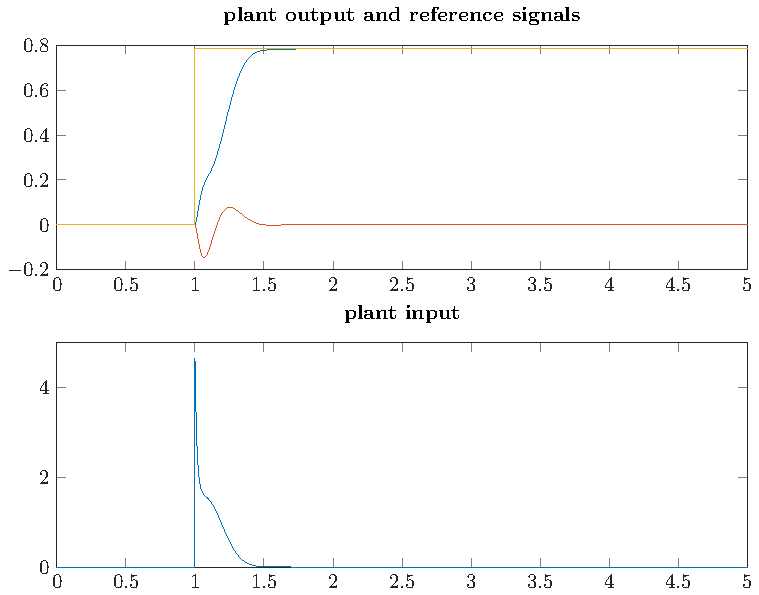
\includegraphics[scale=0.4]{images/orgFullState.pdf}
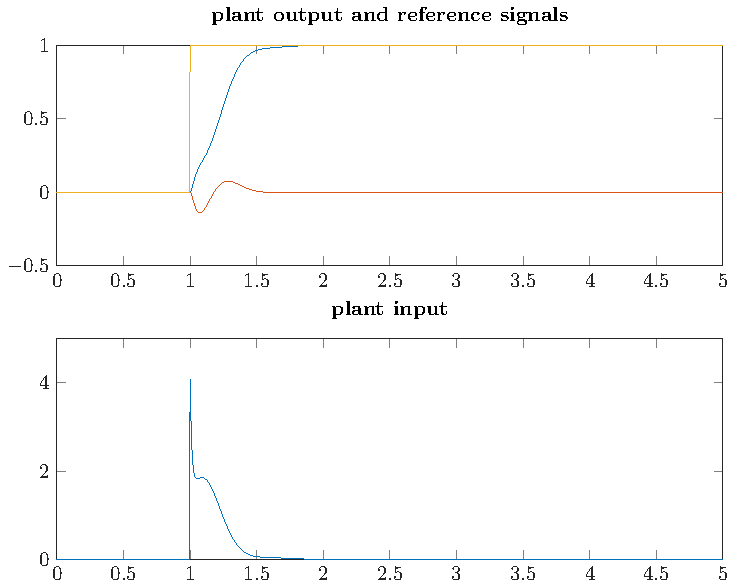
\includegraphics[scale=0.4]{images/optFullState.pdf}
\caption{Simulation results for the original weighting parameters left and for the improved weighting parameters right.}
\label{fig:stepResponse}
\end{figure}


\section{Concluding Simulations with filter and differentiator}
\begin{figure}
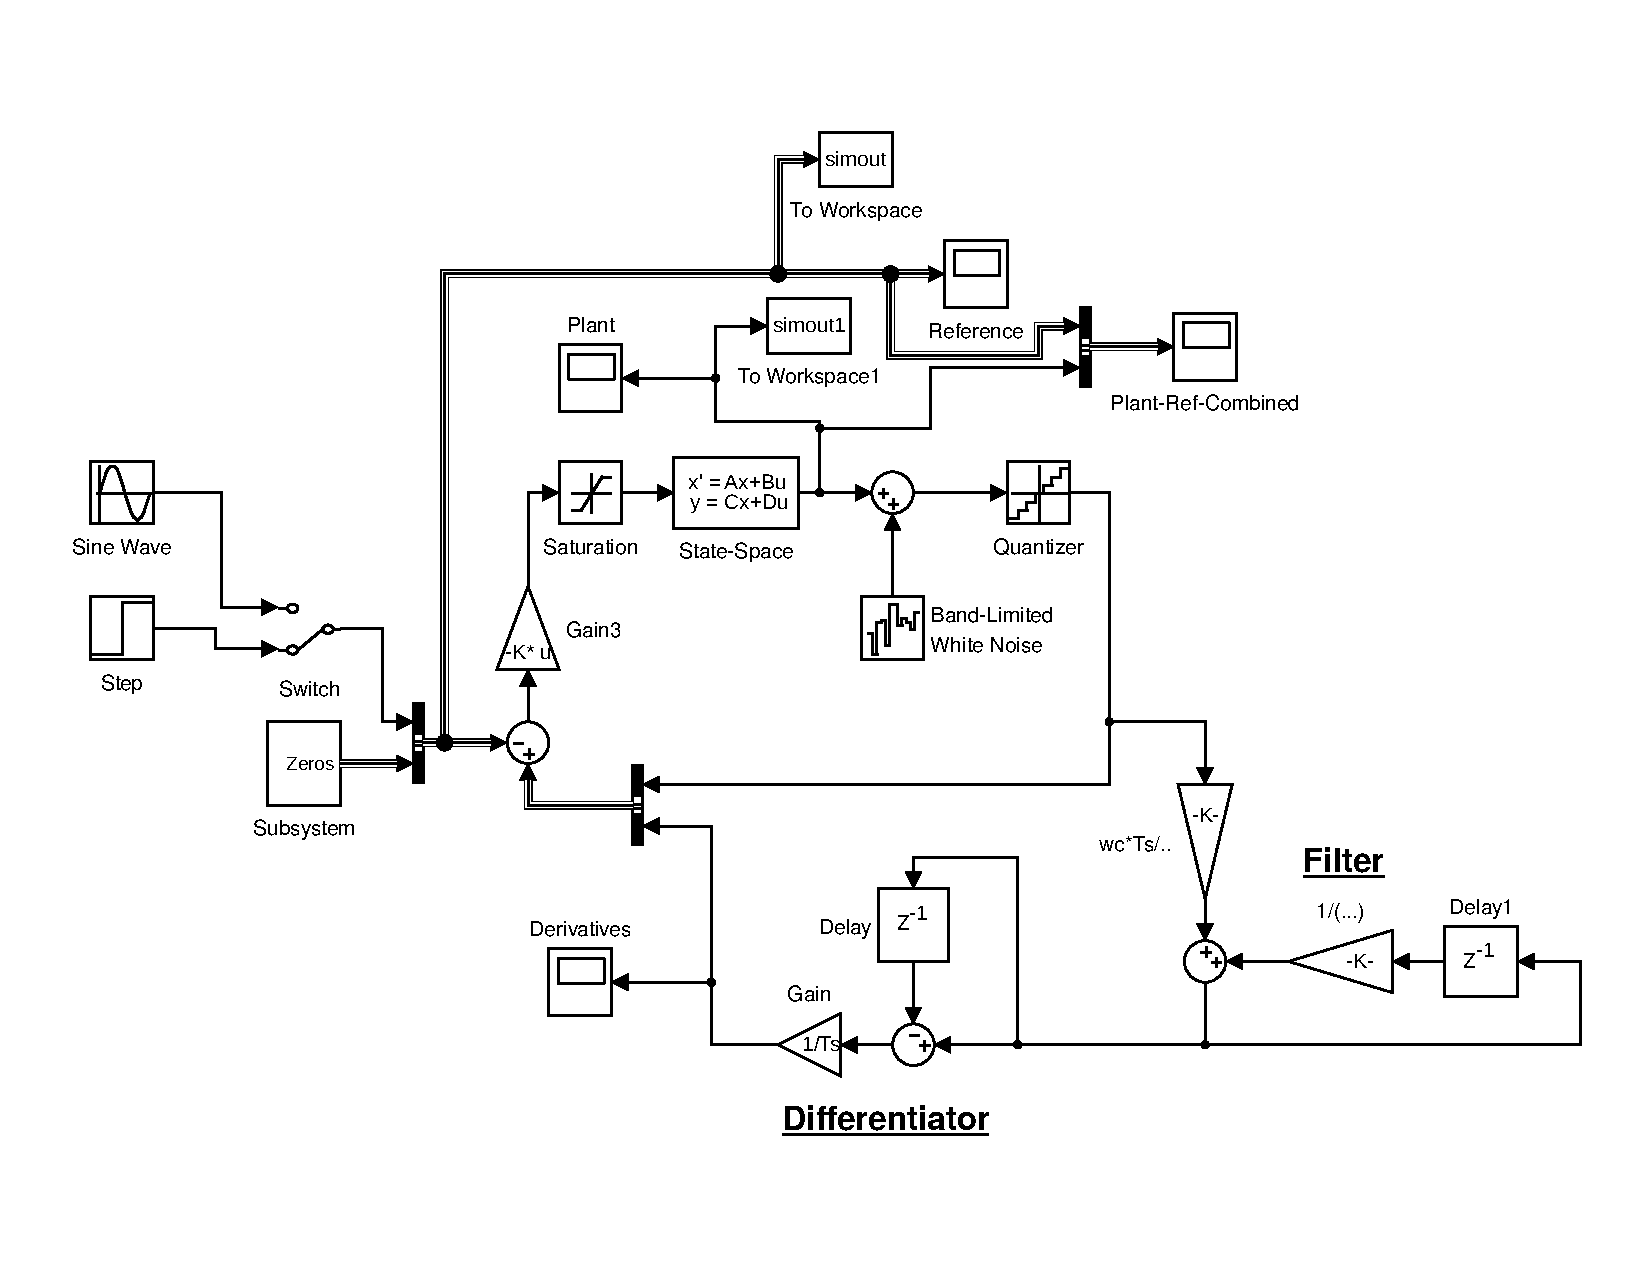
\includegraphics[scale=0.5]{images/simModel.pdf}
\caption{The simulink Layout of our Simulation}
\end{figure}



\section{Tests of the controller on the real setup}

\begin{figure} \label{realtimeSimDiagram}
  \centering
  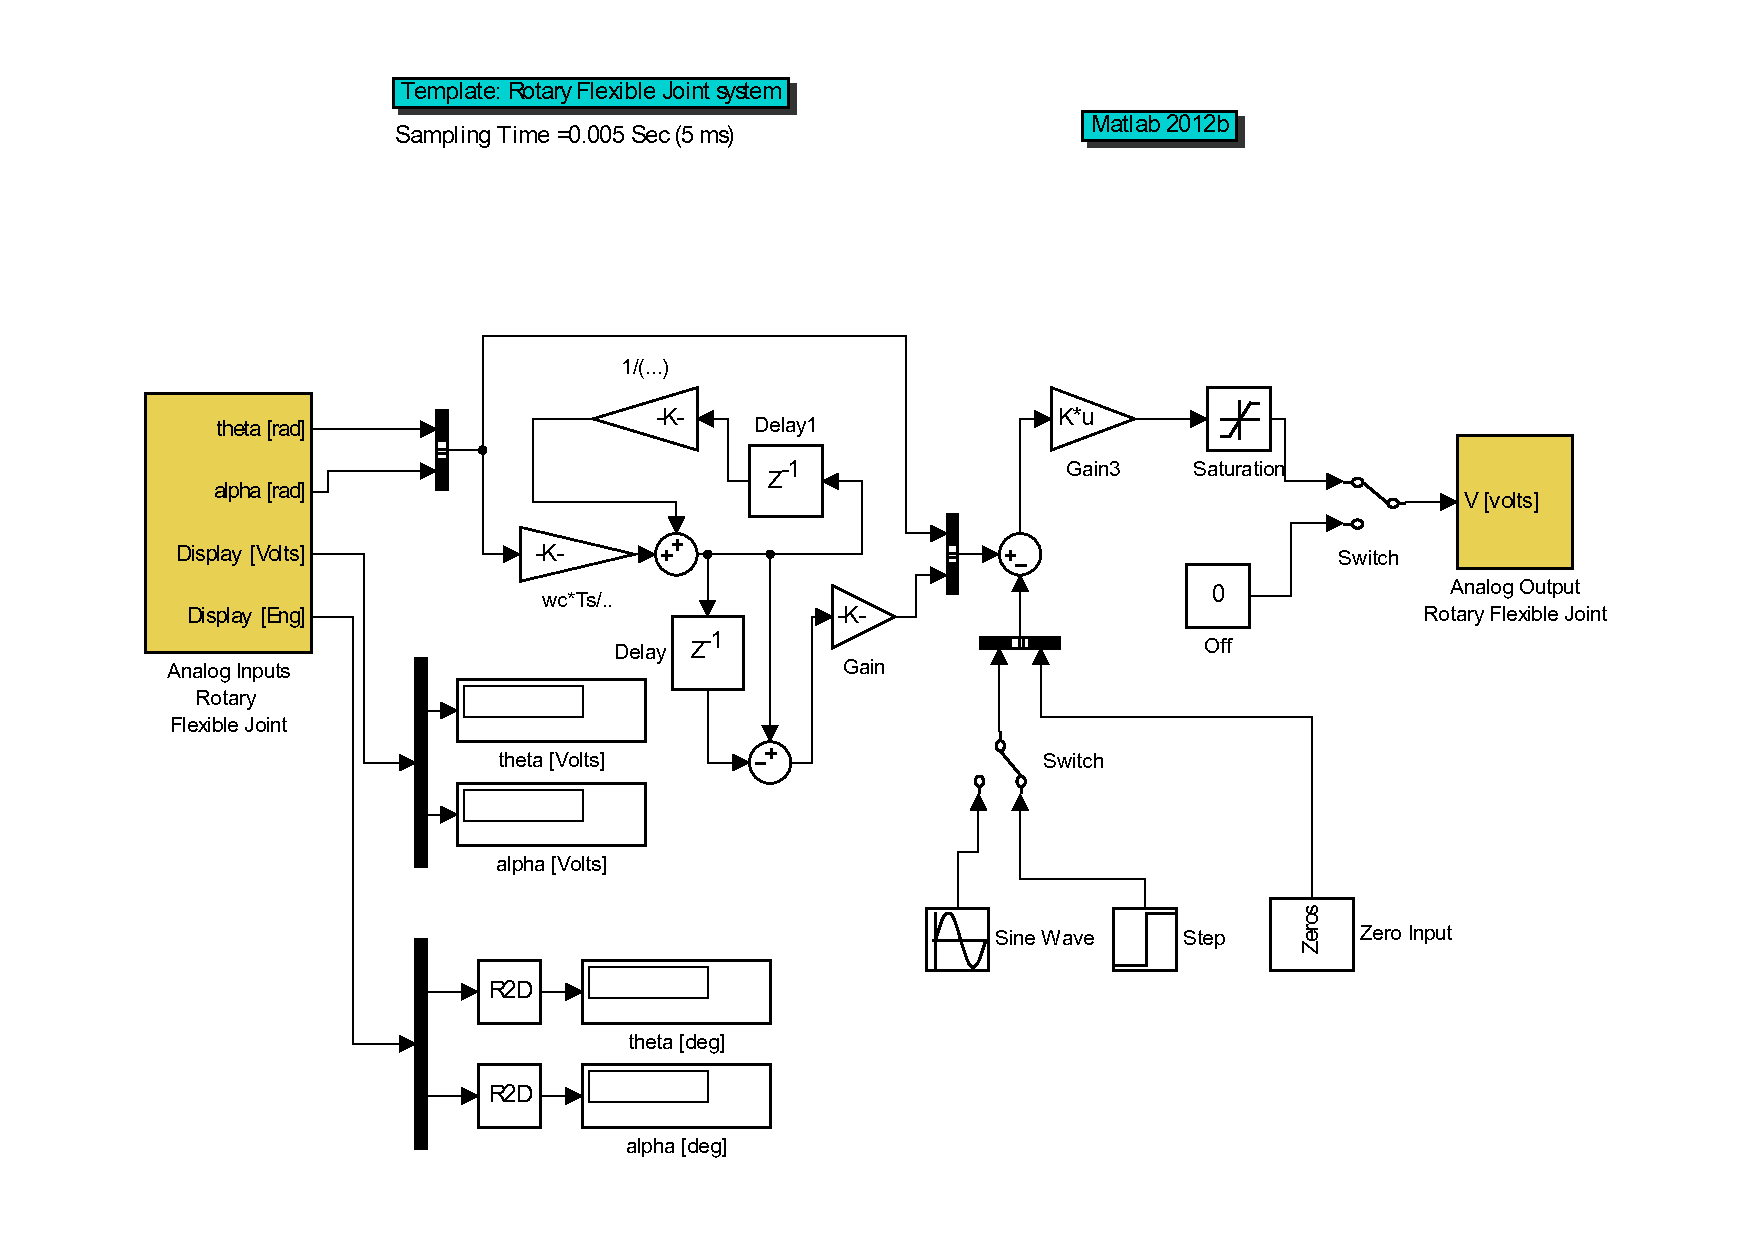
\includegraphics[scale=0.6]{images/realtimeSimDiagram}
  \caption{Real-time Simulink diagram} 
\end{figure}

In figure $\eqref{realtimeSimDiagram}$ we see the real-time Simulink diagram that we used in the lab for the real setup. The "Analog Inputs" block gives the measurements of the sensors (they are updated each 5 ms) in radians for the angles of the hub and the arm. Additionally this block has two special outputs, "Display[volts]" and "Display[Eng]", which are used for visualization purposes. These two outputs are connected to a set of displays in order to provide a local visual measure of the process variables. 

The "Analog Output" block allows the controller to send a voltage signal to the motor of the hub. At the input of this block there is an on-off switch. This switch allows you to switch on or switch off the motor. We included a saturator in our diagram just before the signal goes in to the "Analog Output" block because the output voltage is limited from $-5V$ to $5V$. The saturator settings in our diagram are set accordingly. You can also see a sin wave, a step input and a zero input. These are used to represent a reference signal for the output. The sine wave or the step input is the reference for $\theta_{desired}$ and the zero block are 3 signals equals to zero that represent the reference for $\alpha, \dot{\theta}$ and $\dot{\alpha}$.





\end{document}
